%%% Kapitoly
\chapter{Experimenty}
\label{chap:experimenty}
Všechny práce zmíněné v úvodní kapitole používají evoluční algoritmy k vytvoření řízení chování homogenního robotického hejna, tzn. s jedním druhem robotů. V následující kapitole podrobně popíši postup hledání optimální chování pro heterogenního hejna. Optimalizaci jsem navrhl a otestoval na třech rozličných scénářích. 
\par
\subsubsection{Pracovní názvy scénářů:}
\begin{enumerate}
	\item Wood Scene - zpracování dřeva
	\item Mineral Scene - přetvoření minerálů na palivo 
	\item Competitive Scene - soubojový scénář
\end{enumerate}

Hlavní motivací při tvorbě scénářů bylo vytvořit obtížnější úkoly než se obvykle používají jako například: shlukování, vyhýbání překážkám, atp. Navrhnout je natolik komplexně, aby nebylo možné, že část hejna se nebude podílet na jeho plnění. Také jsem volil scénáře, aby se přiblížily situacím z reálného světa. Každému z nich jsem věnoval samostatnou kapitolu, která zahrnuje popis hlavního úkolu scénáře, seznam robotů i s jejich senzory a efektory, způsob hodnocení fitness,rozdělení do podúkolů s průběhem fitness u ES a DE, vizualizaci a rozbor chování nejlepšího jedince.  
\par
Pro řešení problému jsem navrhl řadu postupů, proto v tomto odstavci zmíním ty nejvíce přímočaré a slibné, které se ovšem ukázaly  jako neúspěšné. V kapitolách zabývajícími se konkrétními scénáři už budu pouze popisovat jen konečné, úspěšné postupy.
\par
Nedostatečný se ukázal pokus provádět evoluci pro fitness hlavního úkolu scénáře. Konkrétně pro Wood Scene počet natěženého a uskladněného dřeva, pro Mineral Scene objem vytvořeného paliva, pro kompetitivní scénář zbylé body zdraví a udělené poškozený. Většina hodnocení náhodných chování byla rovna nule, proto EA nedostaly dostatek informací k vhodné exploraci a díky malé pravděpodobnosti vygenerování chování alespoň částečně řešící hlavní úkol nedocházelo ani k exploataci. Což mělo za důsledek neefektivní  DE a ES, takže ani jeden z EA nedošel k úspěšnému řešení. 
\par
Posun zaznamenala více obecná fitness i když sama o sobě také nedosáhla do kategorie úspěšných postupů. Do fitness jsem zahrnul i menší pozitivní znaky, které byly součástí hlavnímu úkolu. Například jsem záporně ohodnotil pokusy o pohyb končící kolizí, kladně počet nalezených entit či vhodných objektů v kontejnerech, aktuální stav paliva. Optimalizovaná chování opravdu zaznamenala posun. Ovšem oba EA obtížně hledaly cestu z lokálního optima a ve většině případů optimalizovali pouze jednoduché části úkolu. I přes přidávání složitějších matematických funkcí do fitness nebyly schopny dosáhnout uspokojivého řešení hlavního úkolu scénáře.  
\subsubsection*{Nějak pojmenovat}
Pro finální řešení jsem zvolil metodu, kterou nazývám metodou podúkolů. U každého scénáře podrobně popíši její průběh a nastavení, zde pouze nastíním základní  myšlenku. Rozdělil jsem hlavní cíl na několik menších podúkolů (metaúkolů). Každému z nich vytvoříme fitness funkci odpovídající nutné části hlavního cíle. Fitness metaúkolu jsem navrhoval, tak aby necílila na již optimalizované úkony a v každém podúkolu jsem se vždy soustředil pouze na jeden jednoduchý úkon. Díky tomuto principu jsem dosáhl mnohem vyšší odolnosti proti uvíznutí v lokálním minimu. Explorace se tímto procesem také zlepšila, protože hlavní cíl závisí na podúkolech a pokud bylo chování rozmanité a úspěšné, přenesly se tyto vlastnosti i dále. Poté jsem generaci úspěšnou v průzkumu optimalizoval na sbírání materiálů pouze požadované barvy a takto jsem rozděloval až k finálnímu úkolu scénáře. 
\par 
Každý robot má připojen paměťový slot, neboť roboti s nimi dosahovali ve všech úkolech znatelně lepších výsledků a pomáhaly vytvářet složitější chování. 
\section{Použité technologie}
Tuto kapitolu věnuji klíčovým technologiím, jenž jsem použil pro modelování řešeného problému a optimalizaci náhodných chování. Pro ovládání robotů jsem zvolil v poslední době velmi oblíbené \textit{neuronové sítě}, které se často používají v kombinaci s EA. Jednomu jedinci odpovídá jedna neuronová síť ovládající všechny části robota. Tyto neuronové sítě si lze představit jako vektor reálných čísel, což je vhodná reprezentace genotypu pro EA. 
\subsection*{Reprezentace Chování - neuronové sítě}
Pro reprezentaci jedinců v oblasti robotiky, rozpoznávání obrazů a dalších oblastí umělé inteligence se v poslední době používají nejčastěji neuronové sítě. Neuronová síť se strukturou podobá neuronovým sítím v mozku. Základní sítě se skládají z jednotlivých neuronů, které se v kontextu informatického světa nazývají \textit{perceptrony}. Samostatný perceptron je sám o sobě také neuronovou sítí, ale většinou se propojují do složitějších struktur. Perceptron lze definovat podle \citep{neuron} následovně.
\begin{definice}[Perceptron] Perceptron je funkce z $\mathbb{R}^n \rightarrow \mathbb{R}$, která je dáná následujícím předpisem: 	$Y = S(\Theta + \sum_{i=0}^{n} w_i x_i)$, kde pro $i \leq n$ $x_{i}$ je $ítý$ prvek vstupního vektoru, $w_{i}$ se označuje jako váha a většinou $w_{i} $ se bere z $\mathbb{R}$.  $\Theta$ se nazývá práh (bias) a slouží jako váha s konstantním vstupem 1.  $S(X)$ je aktivační funkce: $\mathbb{R} \rightarrow \mathbb{R}$ a $Y$ se obvykle označuje jako výstup perceptronu.
\end{definice}
\textit{Jednovrstvou neuronovou sítí} pak myslíme n perceptronů, tedy funkci $\mathbb{R}^{n} \rightarrow \mathbb{R}^{n}$, kde $ítou$ složku výstupního vektoru dostaneme aplikací funkce odpovídající $ítému$ perceptronu na vstupní vektor.
\improvement{Přidat část o aktivačních funkcích}
\par
Pokud zapojíme z výstupu jednoho perceptronu na vstup jiného, vznikne \textit{vícevrstvá neuronová sít}. Což znamená, že podmnožiny výstupů z první vrstvy neuronů neurčují přímo výstup, ale jsou opět zvoleny jako vstupní vektory pro další jednovrstvou neuronovou síť. Tímto postupem můžeme vytvářet velmi komplexní struktury.
\par
Skrytá vrstva (hidden layer) je taková jednovrstvá neuronová síť, jejíž výstup(resp. vstup) je pouze vstupem(resp. výstup) jiných perceptronů.
\par
\improvement{přeformulovat??}
Pro mé účely se jsem testoval řadu různých variant neuronových sítí, ale nejvíce se mi osvědčilo následující nastavení, které poskytovalo uspokojivé výsledky a rozumné časové nároky. 
\par 
Jako aktivační funkce jednotlivých perceptronů se mi nejvíce osvědčila často používaná funkce hyperbolického tangentu se změněným oborem hodnot pro konkrétní výstup.
\par
V rámci testovaní jsem zvolil jednoduchou architekturu jednovrstvé neuronové sítě, což se ukázalo jako dostatečné pro uspokojivé řešení jednotlivých scénářů. Jejich architektura je následující. Pro každé reálné číslo, které očekává robot jako vstup pro efektor, byl připojen perceptron do kterého vstupuje vektor reálných čísel odpovídající vektoru všech hodnot přečtených ze senzorů.  Pro dosažení lepších řešení by zde bylo možné nasadit NEAT algoritmus či hledat více specifičtější architektury.Případně vyzkoušet vliv vícero vrstev. \improvement{Přidat do diskuze}
\subsection*{Evoluční algoritmy}
Neuronovou sít si lze představit jako množinu vektorů, kde jeden perceptron odpovídá vektoru reálných čísel (vah vstupů + práh $v =(x_0,x_1...x_n,\Theta)$. V kontextu evolučních algoritmů se pro optimalizaci vektorů reálných čísel nejčastěji používají ES a DE, I z tohoto důvodu jsem zvolil zmíněné algoritmy jako zástupce pro optimalizaci chování heterogenní skupiny robotů. Oba zmíněné algoritmy důkladně popisuji v kapitole \ref{sec:DE} a \ref{sec:ES} a má implementace se od popisu v úvodu liší pouze v malý detailech. Do detailu si je lze prohlédnout v přiložené dokumentaci a kódu. 
\par
V rámci testovaní jsem vyzkoušel mnoho různých nastavení parametrů EA. V tabulce \ref{tab04:nastaveníEA} jsou uvedeny nakonec použité parametry, které dosahovali v experimentech největších úspěchů. \improvement{Popsat co jednotlivé parametry dělají??}Jedná se o tradičně používané parametry, osvědčené v řadě optimalizačních problémů. 
\begin{table}[h]\centering
	\begin{tabular}{l@{\hspace{1.5cm}}D{.}{,}{3.2}D{.}{,}{1.2}D{.}{,}{2.3}}
		\toprule
		 \textbf{differenciální evoluce}\\
		\midrule
		F:     & 0.8 \\
		CR:  & 0.5 \\
		\toprule
		\textbf{evoluční strategie}\\
		\midrule
		alpha & 0.05 \\
		sigma & 0.1\\
		\bottomrule
		\multicolumn{2}{l}{}
	\end{tabular}
	\caption{Nastavení parametrů u EA}
	\label{tab04:nastaveníEA}
\end{table}
\newpage
\section{Wood Scene experiment}
Vzorem Wood Scene scénáře byla těžba dřeva, představme si dřevorubce s motorovou pilou a silné dělníky nakládající zpracované stromy do transportérů a svážející materiál na společnou hromadu. Roboti odpovídají těmto lidským rolím, samozřejmě je jejich činnost značně zjednodušena. V obou případech je cílem maximalizovat počet zpracovaného dřeva na daném místě, což vyžaduje od obou druhů agentů spolupráci. \par
Robotické hejno se ve Wood Scene snaží natěžit a převést, co největší množství dřeva na místo označené rádiovým signálem. Rádiové senzory poskytují robotům sílu signálu a vysílaný kód. Pro místo určené na kupení dřeva je určen unikátní kód 2 a je umístěn doprostřed mapy. Žádný jiný rádiový vysílač vysílající signály s kódem 2 se na mapě nenachází.  
\par
Celé hejno čítá 9 robotů, jedná se o dva různé druhy, které se liší velikostí, rychlostí, senzory i efektory. Na začátku experimentu jsou náhodně rozmístěny do středu mapy na stejném místě jako se rozprostírá skladovací prostor. Dále jsou na mapě náhodně umístěny stromy. Robot v kontextu scénáře nazývaný Scout odpovídá \uv{dřevorubci} v teoretickém vzoru, pohybuje se rychle, má menší rozměry, umí nalezený strom zpracovat na dřevo pro komunikaci má přidělený unikátní kód 0. Oproti tomu robot \uv{dělník} se pohybuje pomaleji, je větší, neumí zpracovávat stromy, ale disponuje nakladačem (vykladačem) a kontejnerem na 5 objektů. 
 \par 
Souhrnně hejno musí strom nalézt, přepracovat na dřevo, poté naložit a odvézt do středu. Celý tento proces zahrnuje typické úkoly pro robotický swarm jako rozprostření, vyhýbání se překážkám, komunikaci mezi jednotlivými agenty, nalezení cesty apod. Z návrhu je zřejmé, že na procesu se musí podílet oba druhy robotů.
\par
V rámci bakalářské práce byla připraven program zajišťující jednoduchou vizualizaci chování robotů. Jeho vizuální výstup můžete vidět na obrázku \ref{obr04:WoodSceneRandomStart}. Na ní si vysvětlíme jednotlivé entity nacházející se na mapě. Mapa je ohraničena obdélníkovou hranicí a chová se jako zeď. Zelené kroužky znázorňují stromy, které ještě nebyly objeveny. Objevený strom změní barvu na žlutou. Modře označený prostor je určen pro uskladnění zpracovaného dřeva, roboti jej zaznamenají jako rádiový signál. Hnědá kolečka zastupují pokácené dřevo. V některých podúkolech se objevuje dřevo už při inicializaci, proto ještě neobjevené má tmavší barvu a objevené světlejší. Pro roboty je v tomto prostoru vysílán rádiový signál. Roboti jsou vyplněny červenou barvou, jejich senzory a efektory mají černou barvu. Pro každý rádiový signál je určena jedna unikátní barva s alfa kanálem. 
\par
Pro potvrzení, že scénář není triviálně řešitelný. Bylo vygenerováno tisíc náhodných chování. Hodnoceny byly dle fitness funkce podúkolu kooperace popsaný níže. Nejlepší z nich můžete vidět těsně po inicializaci mapy \ref{obr04:WoodSceneRandomStart}. Výsledek krátce před 10 000. iterací je zachycen v obrázku \ref{obr04:WoodSceneRandomEnd}. Největší světla zelená plocha je volný prostor, kde se mohou roboti pohybovat. Světle růžový kruh je právě rádiové vysílání, protože všichni roboti vysílají současně je barva celkem sytá. Tmavě fialový kruh označuje místo pro uskladnění, obvykle má modrý odstín, ale protože jej překrývají signály robotů zbarvil se do fialové. Na obrázku \ref{obr04:WoodSceneRandomEnd} vidíme, že se robotům povedlo jeden strom pokácet a dokonce uložit. Většina velkých robotů se dostala do kolize a menší roboti nedokázali objevit ani pětinu stromů.
\begin{figure}[p]\centering
	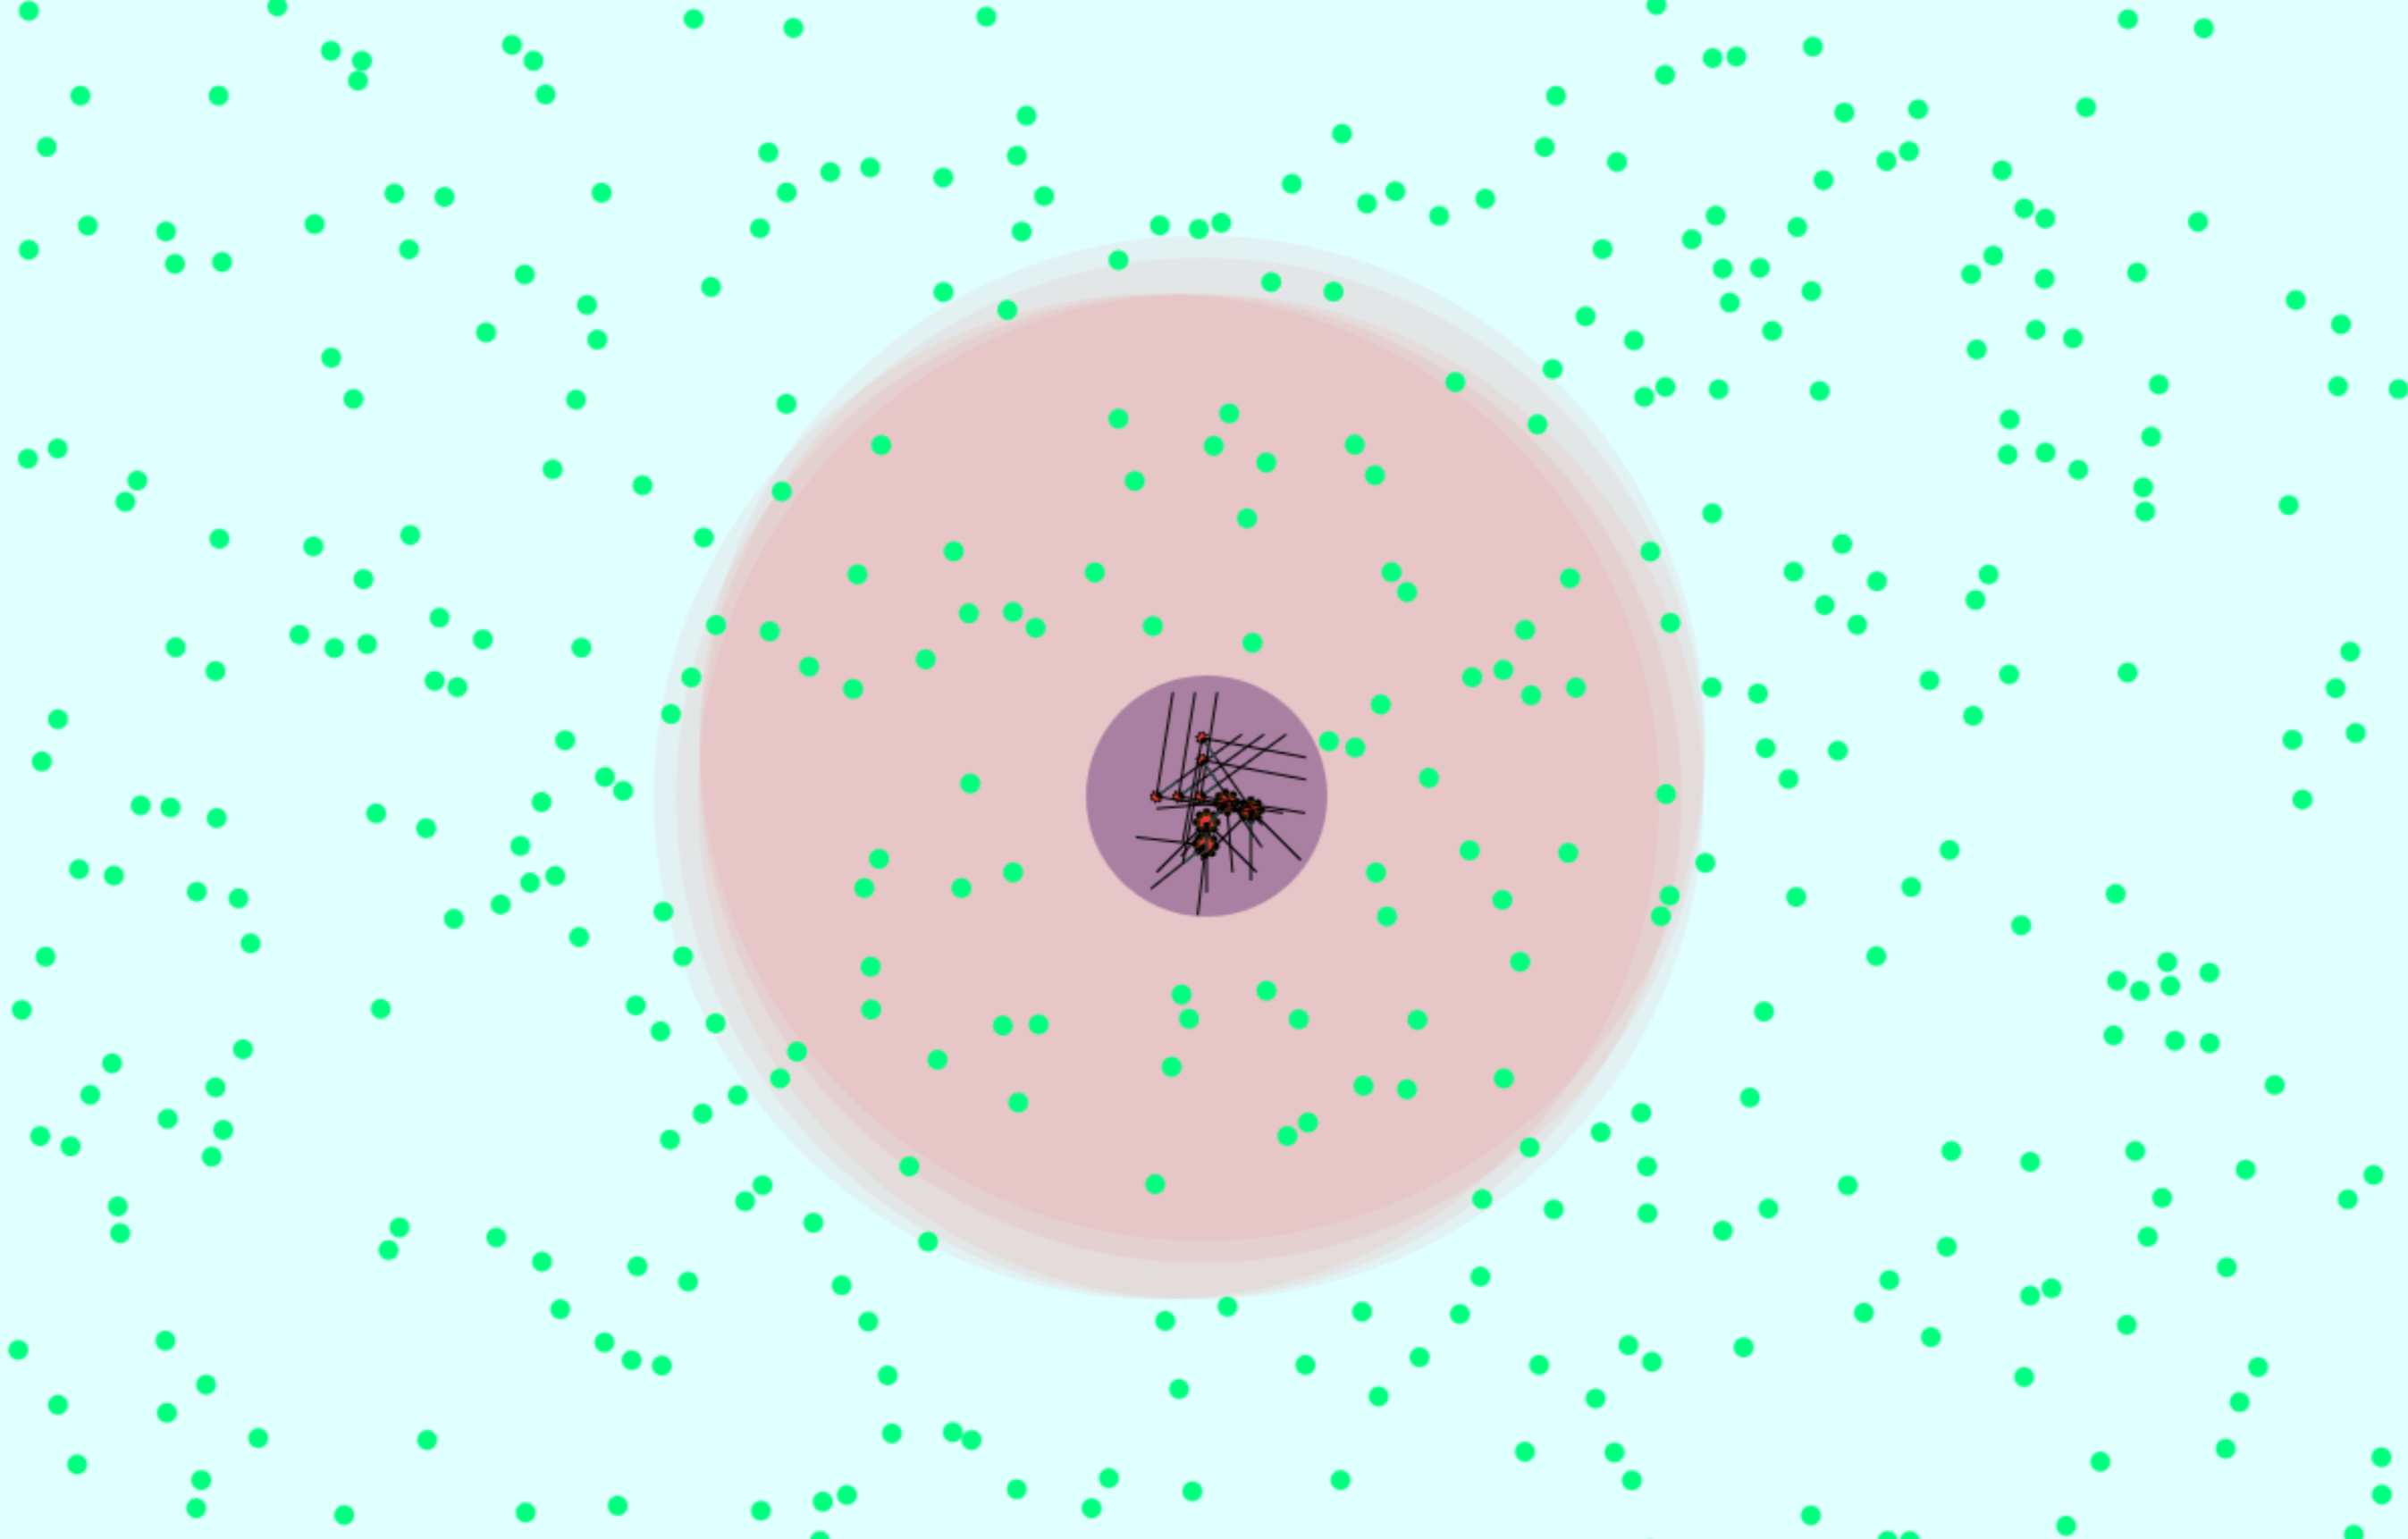
\includegraphics[width=\columnwidth]{../img/WoodMap/pictures/StartRandom.png}
	\caption{Příklad WoodScene mapy: start náhodného chování}
	\label{obr04:WoodSceneRandomStart}
\end{figure}
\par
\begin{figure}[p]\centering
	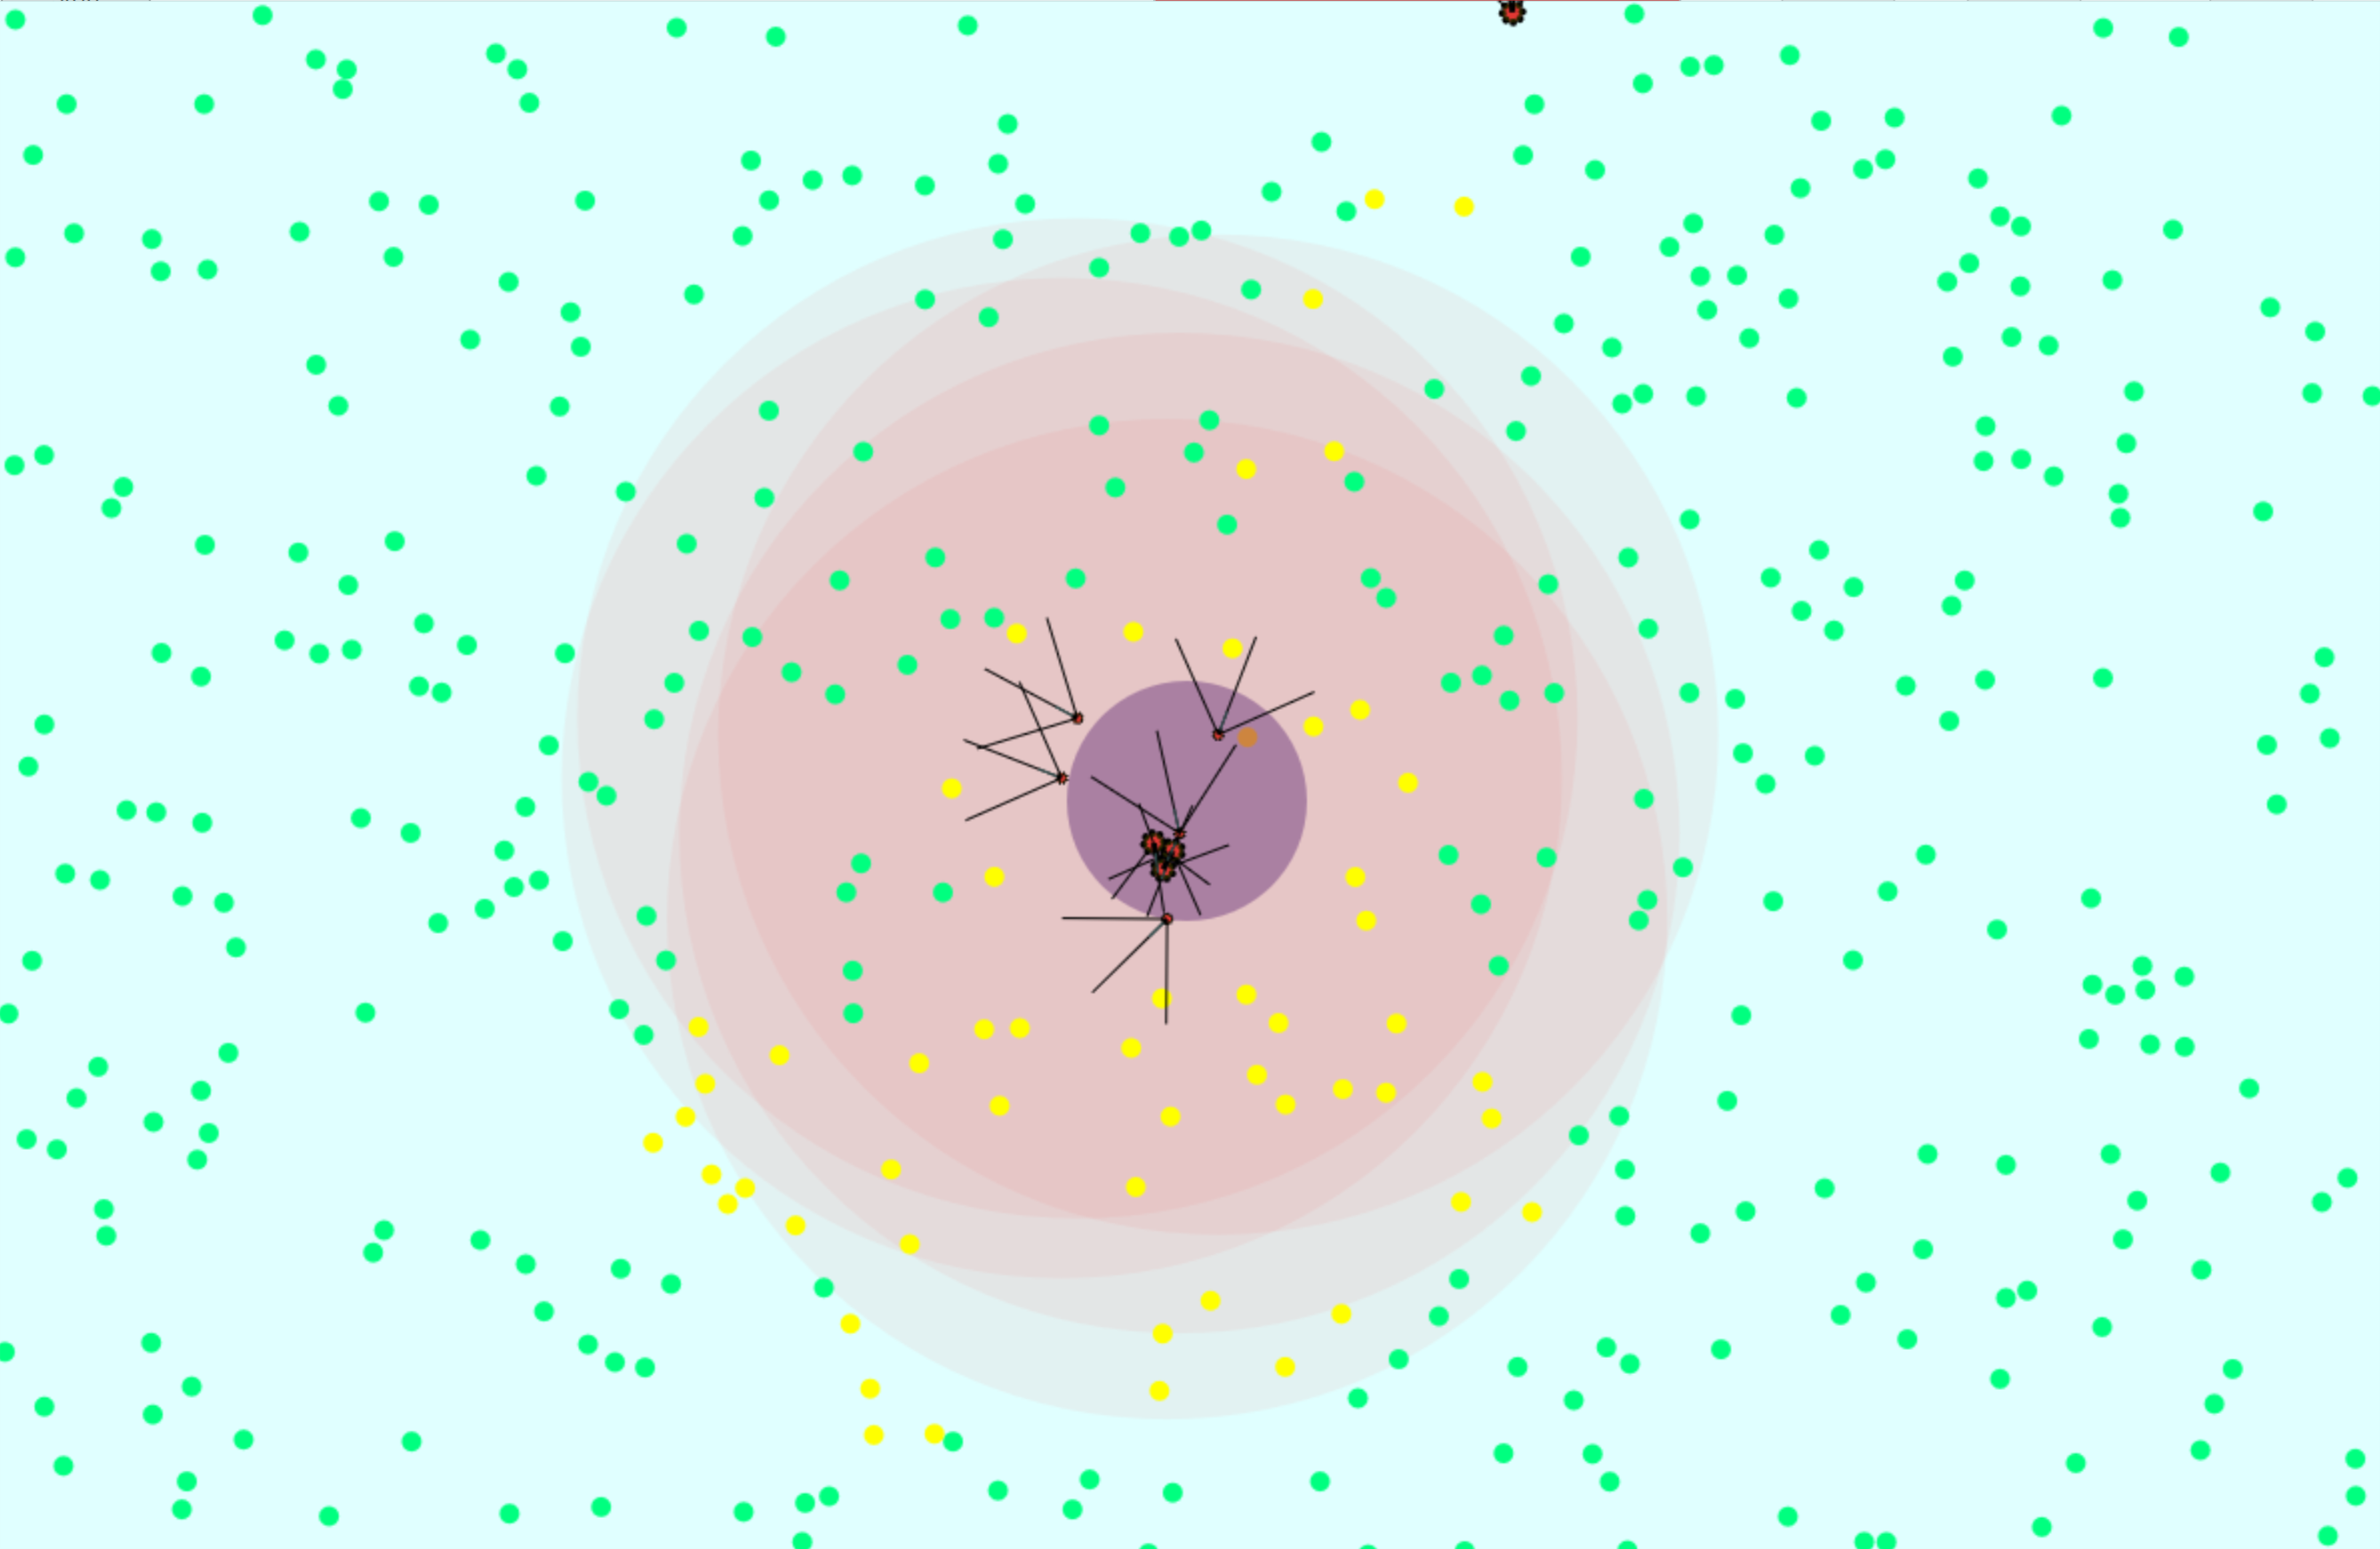
\includegraphics[width=\columnwidth]{../img/WoodMap/pictures/EndRandom.png}
	\caption{Příklad WoodScene mapy: po 9000 iteracích náhodného chování}
	\label{obr04:WoodSceneRandomEnd}
\end{figure}
\clearpage
\subsection{Roboti}
Devítičlenné hejno obsahuje 5 Scout robotů a 4 Worker roboty. U každého z robotů popíši jejich efektory a senzory. Pro každý druh robota je připravena jedna shodná neuronová sít. Jedinec odpovídá vektoru vah neuronové sítě. Pokud v rámci experimentu optimalizuji chování více druhů robotů, jedinec jsou dva vektory vah pro každý druh robota jedna neuronová síť. Proto fitness funkce hodnotí jejich výsledné snažení dohromady a evoluční operátory pracují nad celou dvojicí. Podívejme se na jednotlivé druhy podrobně.
\subsubsection{Scout robot}
Jedná se o robota, který má na starosti průzkum mapy a kácení nalezených stromů. Na zpracování dřeva používá efektor, nazývám jej refaktor, který má podobu úsečky a vyčnívá z čela robota. Pro zpracovaní musí refaktor kolidovat se stromem v mapě, poté je strom prohozen za entitu dřeva. Aby mohl komunikovat má přidělený rádiový signál s kódem 0, při jeho vysílání přidá na mapu signál jako kruh se středem odpovídajícím pozici robota. Jedná se o menšího robota, oproti Worker robotovi je rychlejší a jeho senzory mají větší dosah. Tabulka \ref{tab04:Scout} obsahuje základní charakteristiky, počty a dosahy jednotlivých senzorů a efektorů.
\par 
\begin{table}[h]\centering
\begin{tabular}{l@{\hspace{1.0cm}}D{.}{,}{2.2}D{.}{,}{2.2}D{.}{,}{2.3}}
	\toprule
	\textbf{Scout Robot} \\
	\midrule
        Tvar: & Kruh & \\
        Poloměr: & 2,5 \\
        Název: & WoodCutterM \\
        Velikost kontejneru: & 0\\
        \midrule
        \textbf{Efektory} \\
        \midrule
        Motor: & Dvou kolečkový \\
        Maximální rychlost: & 3 \\
        Kód rádiového signálu: & 0 \\
        Poloměr signálu: & 200\\
        Refaktor: & Strom \Rightarrow Dřevo \\
        Dosah refaktoru: & 10\\
        Počet paměťových slotů: & 10 \\
        Obsah slotu: & float\\
        \midrule 
        \textbf{Senzory} \\
        \midrule
        Počet line senzorů: &  3 \\
        Délka line senzorů: & 50\\
        Orientace line senzorů: & 0^\circ, 45^\circ, -45^\circ \\
        Poloměr type senzoru: & 50\\
        Poloměr rádiového přijímače: &  100 \\
        Počet touch senzorů: & 8 \\  
        Lokátor senzor\\ 
	\bottomrule
	\multicolumn{2}{l}{}
\end{tabular}
\caption{Wood Scene - Scout robot popis}
\label{tab04:Scout}
\end{table}
\clearpage
\subsubsection{Worker robot}
Worker robot se stará o manipulaci a následný transport objektů na mapě. Pohybuje se pomaleji než Scout a také je o něco rozměrnější. Picker, úsečkový efektor sloužící pro nakládání a vykládání objektů, funguje na podobném principu jako refaktor pro naložení musí kolidovat s objektem a pro vyložení s ním nesmí nic kolidovat. Ke komunikaci mu byl vyhrazen rádiový signál s kódem 1. Sebrané objekty ukládá do kontejneru, kam se vejde celkem 5 entit a vykládat umí pouze entitu na vrchu. Tabulka \ref{tab04:Worker} popisuje další podrobnosti.
\par 
\begin{table}[h]\centering
	\begin{tabular}{l@{\hspace{1.0cm}}D{.}{,}{2.2}D{.}{,}{2.2}D{.}{,}{2.3}}
			\toprule
			\textbf{Worker Robot} \\
			\midrule
                Tvar: & Kruh\\
                Poloměr: & 5\\
                Název: & WoodWorkerM \\
                Velikost kontejneru: & 5\\
                \midrule
                \textbf{Efektory} \\
                \midrule
                Motor: & Dvou kolečkový \\
                Maximální rychlost: & 2 \\
                Kód rádiového signálu: & 0\\
                Poloměr signálu: & 200\\
                Dosah pickeru: & 10\\
                Počet paměťových slotů: &10 \\
                Obsah slotu: & float\\
                \midrule 
                \textbf{Senzory} \\
                \midrule
                Počet line senzorů: &  3\\
                Délka line senzorů: & 30\\
                Orientace line senzorů: & 0^\circ, 45^\circ, -45^\circ\\
                Poloměr rádiového přijímače: & 100 \\
                Počet touch senzorů: & 8 \\  
                Lokátorový senzor\\ 
	\bottomrule
\multicolumn{2}{l}{}
\end{tabular}
\caption{Wood Scene - Worker robot popis }
\label{tab04:Worker}
\end{table}
\clearpage
\subsection{Vyhodnocování Fitness}
Fitness funkce pro ohodnocení WoodScene scénáře probíhá vždy až na konci simulace. I když se úspěšnost v podúkolech  vždy posuzuje jinak, celou fitness funkci lze shrnout do následujícího cílů. Roboti jsou odměňováni za: 
\begin{enumerate}
        \item \textit{nalezené stromy} - stromy o které zavadil line senzor 
        \item \textit{pokácené stromy} - stromy, které refaktor změnil 
        \item \textit{sebrané dřevo} - zpracované dřevo, které mají roboti uvnitř kontejnerů 
        \item \textit{uskladněné dřevo} - dřevo, které dovezli na vyznačené místo 
\end{enumerate}
Trestáni za:
\begin{enumerate}
	\item \textit{kolize} - počet pokusů o pohyb při kterém by došlo ke kolizi 
	\item \textit{sebrané entity mimo dřevo} - počet entit v kontejnerech, které nejsou zpracované dřevo 
\end{enumerate}

\subsection{Podúkoly} 
Rozdělil jsem hlavní cíl na následující podúkoly. Jejich obtížnost postupně roste a finální metaúkol už odpovídá řešenému problému. Pro ES a DE jsem použil stejné, abych bylo možné porovnat jejich fungování. 
\begin{enumerate}
        \item vygenerování robotů = Na začátku je vygenerováno chování robotů naprosto náhodně. Pro každého robota, je vygenerována náhodná jednovrstvá neuronová síť. 
        \item učení chůze = Pro oba roboty je velmi důležité, aby se pohybovali bez kolizí po celé mapě a objevovali, co největší prostor. Roboti jsou vyvíjeni odděleně a fitness se soustředí na počet kolizí (záporným ohodnocením) a na nalezené stromy (kladným ohodnocením).
        \item těžba stromů = Scout roboty, kteří se už obstojně po mapě pohybují, je třeba naučit kácet stromy. Proto dalším  cílem ve fitness funkci je počet pokácených stromů. Nicméně stále také na počet stromů nalezených. 
        \item převoz dřeva = Správně pohybující chceme naučit sbírat vytěžené dřevo. Fitness hodnotí počet sebraného dřeva, případně i uskladněné dřevo. Na těchto mapách jsou už na začátku připraveny pouze entity zpracovaného dřeva.
        \item kooperace = V posledním experimentu, se hodnotí pouze sebrané a uskladněné dřevo. A evolvují se oba druhy robotů současně. 
\end{enumerate}
U každého experimentu uvedu \unsure{nebylo by lepší slovo než myšlenku}myšlenku, tabulku s přesným nastavením a poté graf s průběhem fitness jednotlivých EA plus jejich vzájemné porovnání. ES v rámci mutačních operátorů vytváří několik zmutovaných jedinců a na základě jejich fitness utváří potomka. Vyhodnocování fitness je časově nejnáročnější výpočet, protože se musí probíhat na mapě celá simulace. Aby časy běhu DE a ES byly srovnatelné, odpovídá velikost populace u DE, velikosti populace krát počet mutovaných jedinců u ES. Při porovnání EA zobrazuji průměrné hodnoty fitness jedinců v rámci daného podúkolu. 
\newpage
	\subsubsection{Scout chůze - nastavení experimentu}
	Nejdříve jsem se zaměřil na schopnost pohybu jednotlivých robotů po mapě. Oddělil jsem oba druhy od sebe, protože díky rychlejšímu pohybu Scout robotů EA optimalizovalo pouze jejich pohyb. Roboti byli oceněni za nalezené stromy, tato fitness je nutila rozprostřít se po mapě. Následuje tabulka s nastavením fitness a EA.
	\par
	\begin{table}[h]\centering
		\begin{tabular}{l@{\hspace{1.5cm}}D{.}{,}{3.2}D{.}{,}{1.2}D{.}{,}{2.3}}
			\toprule
			\textbf{Nastavení mapy a EA}\\
			\midrule
			Roboti:     & Scout-5 \\
			Počet generací: & 1000\\
			Počet iterací map & 1000\\
			Velikost generace(DE) & 200\\
			Počet jedinců(ES) & 10\\
			Počet mutovaný potomků(ES)&20\\
			Elitismus(ES)& Ano\\
			Elitismus(DE)& Ne \\
			\bottomrule
			\multicolumn{2}{l}{}
		\end{tabular}
		\begin{tabular}{l@{\hspace{1.5cm}}D{.}{,}{3.2}D{.}{,}{1.2}D{.}{,}{2.3}}
			\toprule
			\textbf{Fitness funkce}\\
			\midrule
			Hodnota nalezeného stromu &  10 \\
			Ostatní hodnoty: & 0\\
			Počet stromů: & 300\\
			Počet už pokácených stromů & 100\\
			\bottomrule
			\multicolumn{2}{l}{}
		\end{tabular}
		\caption{Scout chůze - nastavení experimentu}\label{tab04:ScoutWalk}
	\end{table}
    Výsledky experimentu ilustrují grafy na další stránce. Jednotlivé průběhy fitness na obrázku \ref{obr04:WalkESvsDE} ukazují střední hodnotu fitness a její rozptyl v závislosti na generaci, jedinci jsou kvůli přehlednosti sloučeni po 10 generacích. V obou případech docházelo k největšímu růstu do 200 generace (v grafech 20). Oba EA lze označit jako úspěšné, protože vygenerovaná chování objevila více než 50\% stromů na mapě, v případě DE dokonce více dvě třetiny. U ES jsem nepoužíval elitismus, proto křivka více osciluje než je tomu u DE.
	\begin{figure}[t]\centering
		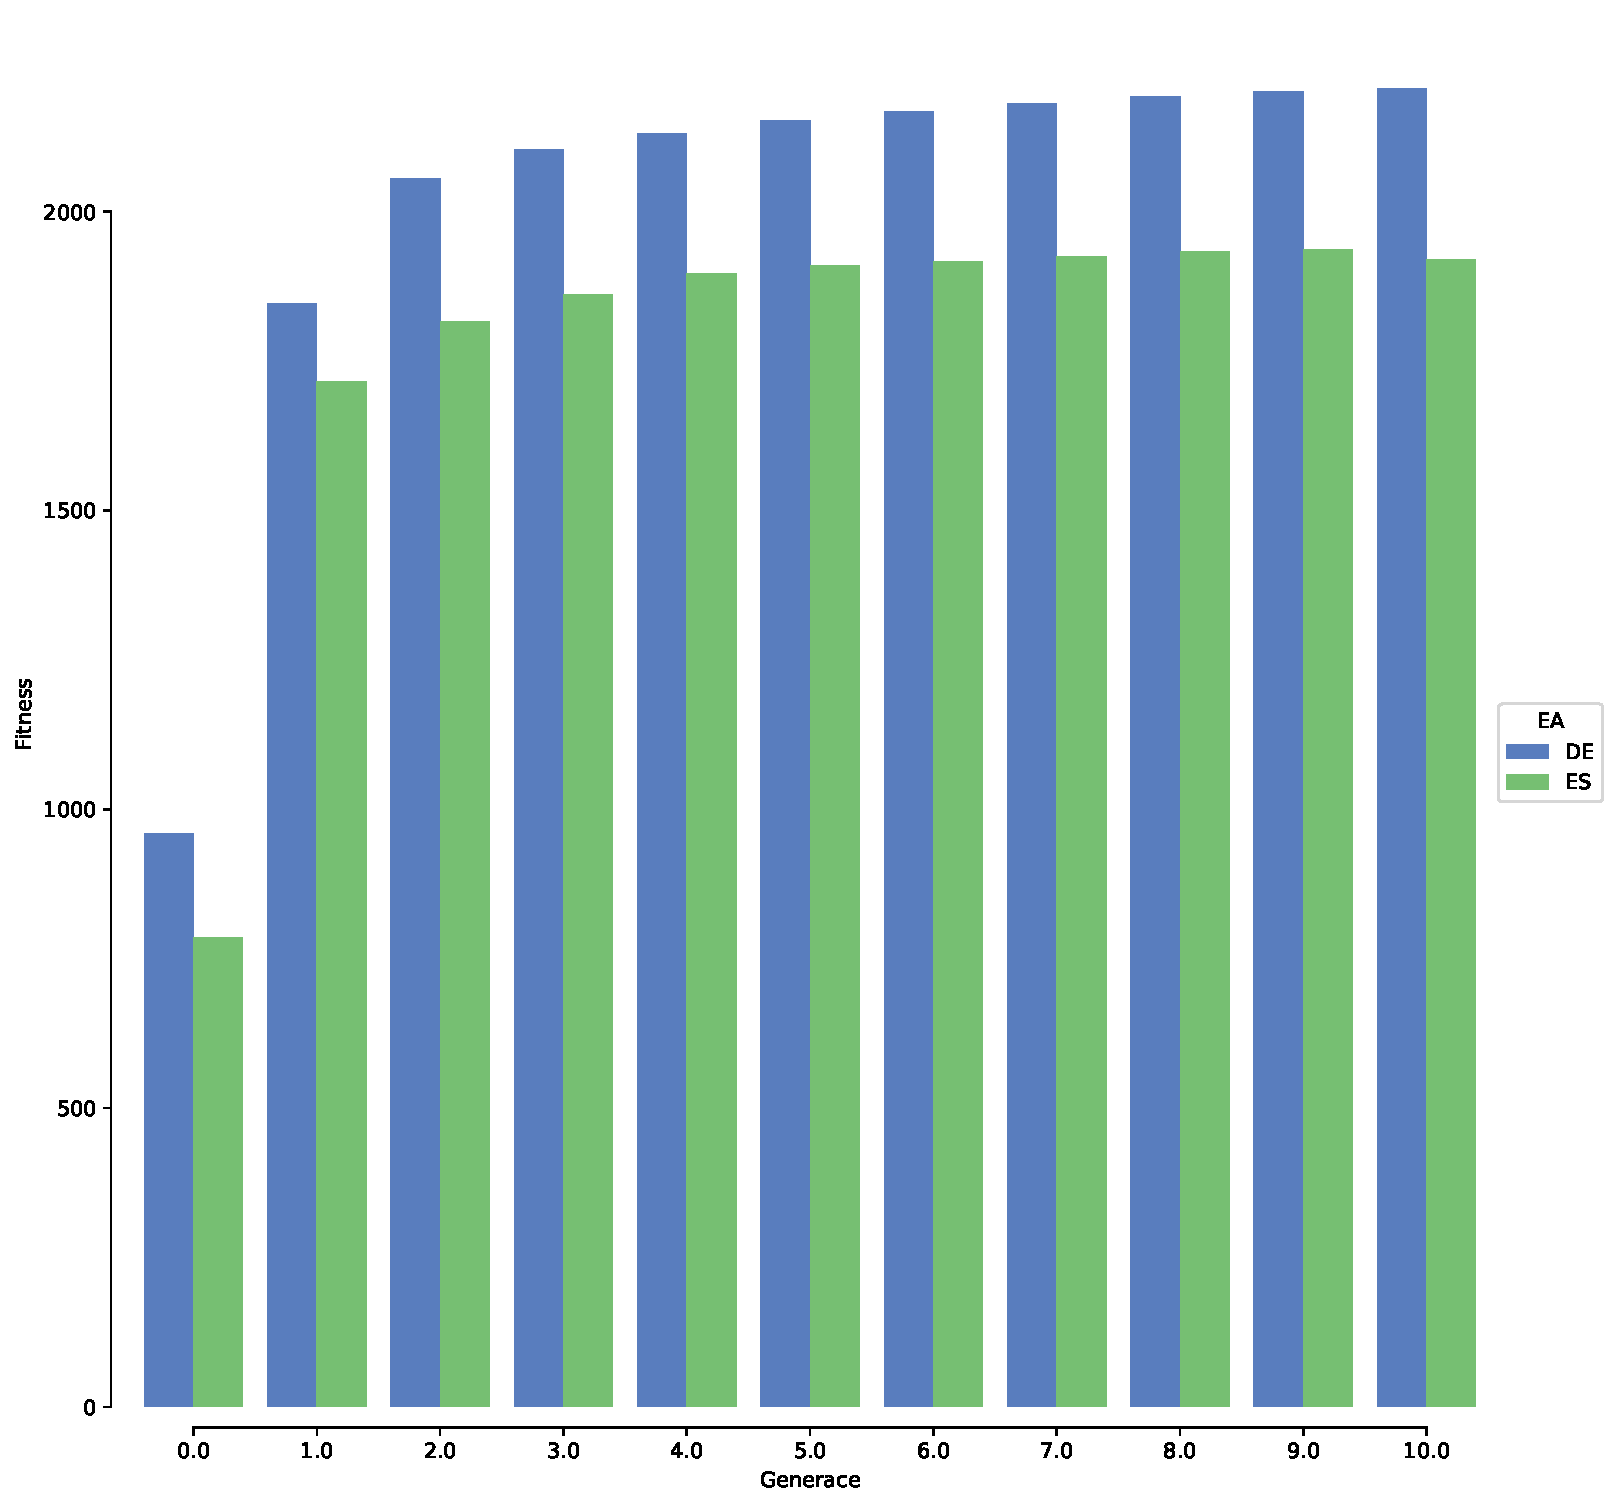
\includegraphics[width=\columnwidth]{../img/WoodMap/DEvsES/WCuttorWalkMem}
		\caption{ Scout chůze - porovnání průměrné fitness ES a DE}
		\label{obr04:WalkESvsDE}
	\end{figure}
	\clearpage
	
	\subsubsection{Worker chůze - nastavení experimentu}
	Worker chůze aplikuje podobný postup jako v předchozím experimentu na Worker roboty. Jen jsem nehodnotil počet nalezených stromů, ale do každé mapy jsem umístil už zpracované stromy. Roboti tedy byli oceněni za nalezení právě tohoto dřeva. Opět fitness funkce nutí roboty, co nejvíce se rozprostřít po mapě a navíc ještě vyhýbat se nepokáceným stromům.
	\par
	 	\begin{table}[h]\centering
		\begin{tabular}{l@{\hspace{1.5cm}}D{.}{,}{3.2}D{.}{,}{1.2}D{.}{,}{2.3}}
			\toprule
			\textbf{Nastavení mapy a EA}\\
			\midrule
			Roboti:     & Worker-4 \\
			Počet generací: & 1000\\
			Počet iterací map & 1000\\
			Velikost generace(DE) & 200\\
			Počet jedinců(ES) & 10\\
			Počet mutovaný potomků(ES)&20\\
			Elitismus(ES)& Ano\\
			Elitismus(DE)& Ne \\
			\bottomrule
			\multicolumn{2}{l}{}
		\end{tabular}
		\begin{tabular}{l@{\hspace{1.5cm}}D{.}{,}{3.2}D{.}{,}{1.2}D{.}{,}{2.3}}
			\toprule
			\textbf{Fitness funkce}\\
			\midrule
			Hodnota nalezeného pokáceného stromu &  20\\
			Ostatní hodnoty: & 0\\
			Počet stromů: & 0\\
			Počet už pokácených stromů & 400\\
			\bottomrule
			\multicolumn{2}{l}{}
		\end{tabular}
		\caption{Worker chůze - nastavení experimentu}
		\label{tab04:WorkerWalk}
	\end{table}
		DE dokázal už ve 200. generaci najít většinu zpracovaného dřevo na mapě, jak můžeme vidět na grafu DE v obrázku \ref{obr04:WWalkESvsDE}. ES neoptimalizovalo v tomto případě příliš rychle a uvízlo v lokalním optimu, jak ukazuje křivka ES od 200. generace. Nejlepší jedinec optimalizovaný pomocí DE byl schopen nalézt až 3x zpracovaného než ten pomocí ES. Nutno dodat, že náhodná pozice se entit na mapě se líší pro ES a DE. Zkoušel jsme, proto měnit seed u generátoru náhodných čísel a výsledky odpovídaly grafům v \ref{obr04:WWalkESvsDE}..
		\begin{figure}[t]\centering
		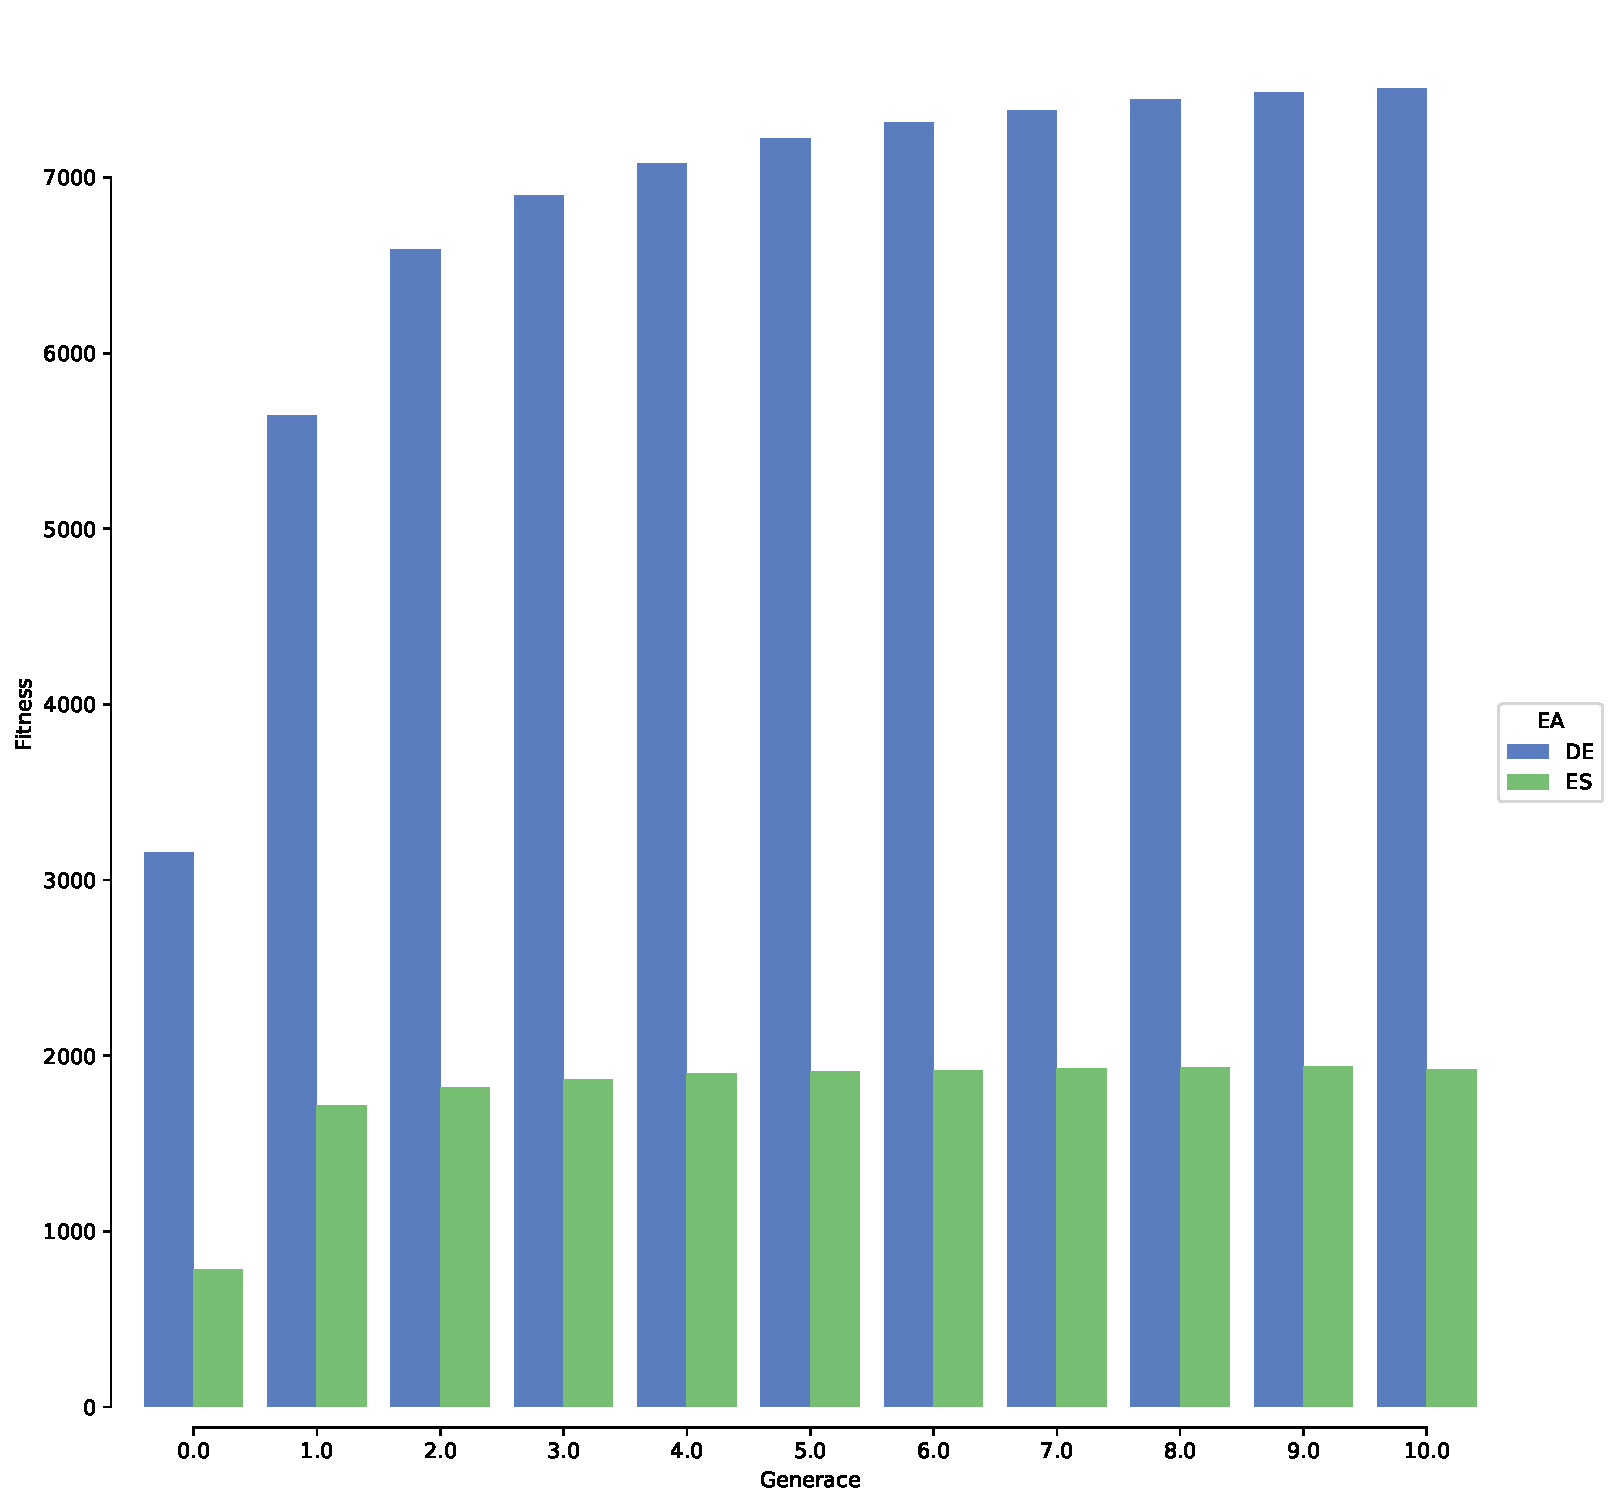
\includegraphics[width=\columnwidth]{../img/WoodMap/DEvsES/WorkerWalkMem}
		\caption{Worker chůze - porovnání průměrné fitness ES a DE}
		\label{obr04:WWalkESvsDE}
	\end{figure}
	\clearpage 
	
	
	
	\subsubsection{Scout kácení - nastavení experimentu}
	Dalším úkolem pro Scout robota bylo nalezené stromy pokácet. Použil jsem tedy optimalizované neuronové sítě z experimentu Scout chůze a tentokrát přidal do fitness pozitivní body za pokácené stromy. Refaktor je o mnoho kratší než line sensory, proto pro kácení musí robot ke stromu přijet blíže. Abych ještě více vylepšil pohyb po mapě, tak každá kolize byla potrestána negativním bodem do fitness. Přesné nastavení obsahuje následující tabulka.
	\begin{table}[h]\centering
		\begin{tabular}{l@{\hspace{1.5cm}}D{.}{,}{3.2}D{.}{,}{1.2}D{.}{,}{2.3}}
			\toprule
			\textbf{Nastavení mapy a EA}\\
			\midrule
			Roboti:     & Scout-5 \\
			Počet generací: & 1500\\
			Počet iterací map & 1000\\
			Velikost generace(DE) & 200\\
			Počet jedinců(ES) & 10\\
			Počet mutovaný potomků(ES)&20\\
			Elitismus(ES)& Ano\\
			Elitismus(DE)& Ne \\
			\bottomrule
			\multicolumn{2}{l}{}
		\end{tabular}
		\begin{tabular}{l@{\hspace{1.5cm}}D{.}{,}{3.2}D{.}{,}{1.2}D{.}{,}{2.3}}
			\toprule
			\textbf{Fitness funkce}\\
			\midrule
			Hodnota nalezeného stromu &  1000\\
			Hodnota pokáceného stromu & 10000\\
			Hodnota kolize & -1\\
			Ostatní hodnoty: & 0\\
			Počet stromů: & 400\\
			Počet už pokácených stromů & 0\\
			\bottomrule
			\multicolumn{2}{l}{}
		\end{tabular}
		\caption{Scout kácení - nastavení experimentu}
	\end{table}
	Dále můžete vidět grafy popisující průběh fitness u DE, ES a porovnání jejich průměrné fitness. Z \ref{obr04:CutESvsDE} můžeme vyčíst, že použité DE více cílí na exploataci a ES na exploraci. DE jsou díky tomu mnohem náchylnější k uvíznutí v lokálním optimu.  Fitness se v tomto případě skládá ze dvou složek, pro jedince bylo mnohem jednodušší stromy objevovat a náhodou nějaké pokácet. V prvních 650 generacích DE se tedy drží tento trend a pak se objeví jedinci, kteří cílí na kácení. Toto chování se rychle rozšířilo a fitness celé populace okolo 700. generace prudce vzrostla. Zatímco fitness v ES rostla postupně, ale nedosáhla tak vysoké úrovně jako DE. Nejlepší jedinci pokácí více než 60\% stromů. 
	\begin{figure}[t]\centering
		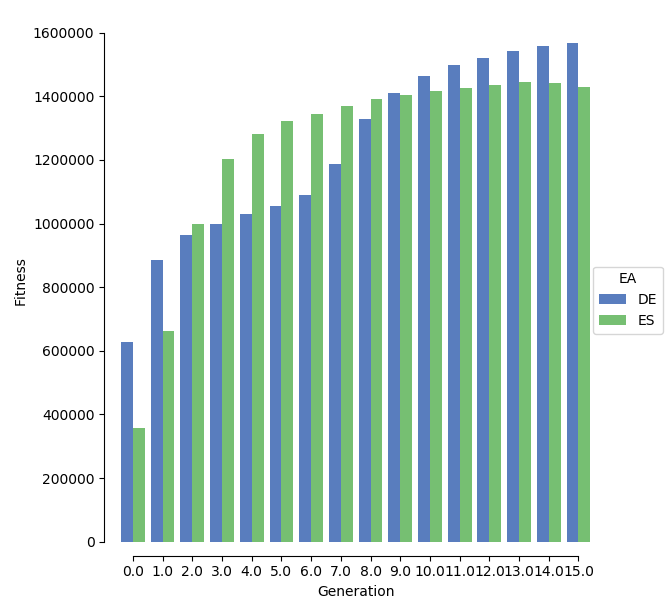
\includegraphics[width=\columnwidth]{../img/WoodMap/DEvsES/WCuttorCutMem}
		\caption{Scout kácení - porovnání průměrné fitness ES a DE}
		\label{obr04:CutESvsDE}
	\end{figure}
	\clearpage
	
	\subsubsection{Worker sbírání - nastavení experimentu}
	Worker v rámci zadání musí řešit více složitý úkol než Scout robot. Celý proces uložení se skládá nejdříve z nalezení dřeva, naložení, poté přesunu místa pro skladování a nakonec vyložení. Optimalizace fungovala lépe po rozdělení na část nakládání, kterou se zabývá tento experiment a na část vykládání, na kterou se podíváme později.  Ve fitness jsem se soustředil na správné entity v kontejneru a na jejich počet. Abych nezahodil dobré chování, které dokáže dřevo i ukládat, za uložení dřeva dostali roboti také pozitivní body. Níže můžete vidět tabulku s konkrétním nastavením. \par
	\begin{table}[h]\centering
		\begin{tabular}{l@{\hspace{1.5cm}}D{.}{,}{3.2}D{.}{,}{1.2}D{.}{,}{2.3}}
			\toprule
			\textbf{Nastavení mapy a EA}\\
			\midrule
			Roboti:     & Worker-4 \\
			Počet generací: & 2000\\
			Počet iterací map & 1000\\
			Velikost generace(DE) & 200\\
			Počet jedinců(ES) & 10\\
			Počet mutovaný potomků(ES)&20\\
			Elitismus(ES)& Ano\\
			Elitismus(DE)& Ne \\
			\bottomrule
			\multicolumn{2}{l}{ }
		\end{tabular}
		\par 
		\begin{tabular}{l@{\hspace{1.5cm}}D{.}{,}{3.2}D{.}{,}{1.2}D{.}{,}{2.3}}
			\toprule
			\textbf{Fitness funkce}\\
			\midrule
			Hodnota nalezeného pokáceného stromu &  100 \\
			Hodnota uloženého dřeva & 1010\\
			Hodnota dřeva v kontejneru & 1000\\
			Hodnota jiné entity v kontejneru & -100\\
			Hodnota kolize & -1\\
			Ostatní hodnoty: & 0\\
			Počet stromů: & 200\\
			Počet už pokácených stromů & 200\\
			\bottomrule
			\multicolumn{2}{l}{}
		\end{tabular}
		\caption{Worker sbírání - nastavení experimentu}
	\end{table}
	V grafech na \ref{obr04:PickupESvsDE} je vidět, že roboti dokázali maximálně naplnit kontejnery zpracovaným dřevem, v případě DE už po 250. generaci zvládala tento úkol celá populace. Chování optimalizované ES mají mnohem větší rozptyl díky vysoké exploraci, ale i její nejlepší jedinci zvládli maximální naplnění již kolem 250. generace. 
		   \begin{figure}[t]\centering       
		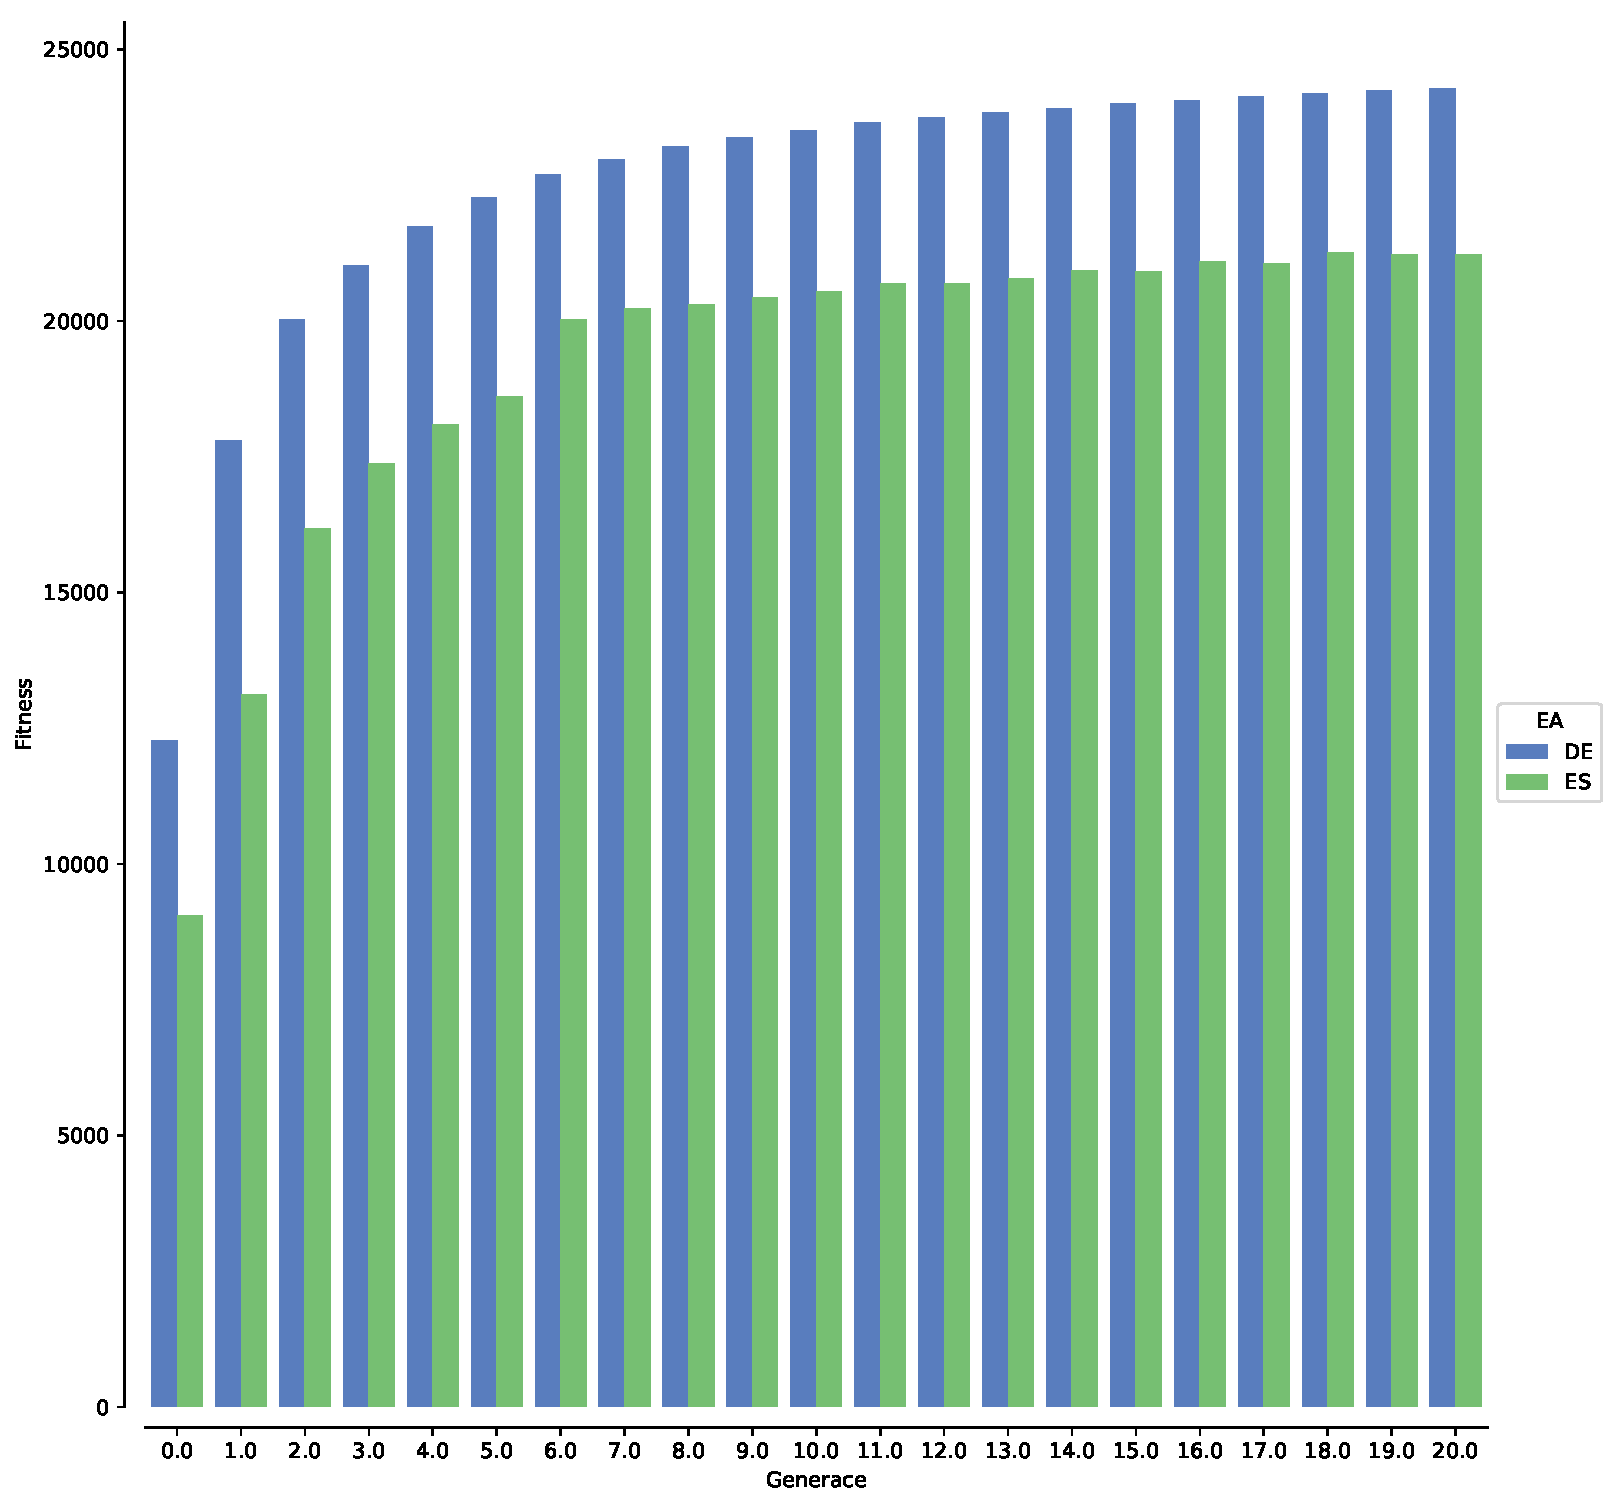
\includegraphics[width=\columnwidth]{../img/WoodMap/DEvsES/WorkerPickUpMem}
		\caption{ Worker sbírání - porovnání průměrné fitness ES a DE}
		\label{obr04:PickupESvsDE}
	\end{figure}
	\clearpage
	\subsubsection{Worker ukládání doprostřed  - nastavení experimentu}
	Ukládání zpracovaného dřeva byl poslední experiment, který plnili Worker roboti samostatně. Zde jsem se soustředil na celý úděl Worker robota a využil už optimalizovaných neuronových sítí na sbírání zpracovaného dřeva z předchozího experimentu. Nejvyšší odměnu roboti získávali za uskladnění dřeva a minoritní odměny za vhodné chování dle předchozích fitness. Vlastním nastavení odpovídá tabulce \ref{tab04:WorkerStore}. \par
	\begin{table}[h]\centering   
		\begin{tabular}{l@{\hspace{1.5cm}}D{.}{,}{3.2}D{.}{,}{1.2}D{.}{,}{2.3}}
			\toprule
			\textbf{Nastavení mapy a EA}\\
			\midrule
			Roboti:     & Worker-4 \\
			Počet generací: & 2000\\
			Počet iterací map & 2000\\
			Velikost generace(DE) & 200\\
			Počet jedinců(ES) & 10\\
			Počet mutovaný potomků(ES)&20\\
			Elitismus(ES)& Ano\\
			Elitismus(DE)& Ne \\
			\bottomrule
			\multicolumn{2}{l}{ }
		\end{tabular}
		\par 
		\begin{tabular}{l@{\hspace{1.5cm}}D{.}{,}{3.2}D{.}{,}{1.2}D{.}{,}{2.3}}
			\toprule
			\textbf{Fitness funkce}\\
			\midrule
			Hodnota nalezeného pokáceného stromu &  100 \\
			Hodnota uloženého dřeva & 1000\\
			Hodnota dřeva v kontejneru & 100\\
			Hodnota jiné entity v kontejneru & -100\\
			Hodnota kolize & -1\\
			Ostatní hodnoty: & 0\\
			Počet stromů: & 200\\
			Počet už pokácených stromů & 200\\
			\bottomrule
			\multicolumn{2}{l}{}
		\end{tabular}
		\caption{Worker ukládání doprostřed  - nastavení experimentu}
		\label{tab04:WorkerStore}
	\end{table}
   	Lokace skladovacího místa působila robotům velké obtíže, proto růst fitness byl mnohem mírnější než u předchozích experimentů. DE dokázala už optimalizované chování rychleji vylepšovat narozdíl od ES, která doplácí na velkou míru explorace viz. \ref{obr04:StockESvsDE}. Nejlepší jedinci jsou ovšem už schopni plnit obstojně hlavní úkol Worker robotů. Objevila se obtíž s efektivním urovnáním zpracovaného dřeva na skladovací místo. Pokoušel jsem se tento problém řešit, přidáním kladných bodů za menší vzdálenost mezi středem skladovacího místa a uloženým dřevem. Nesáhl jsem, však lepších výsledků než v tomto experimentu. 
	\begin{figure}[t]\centering
		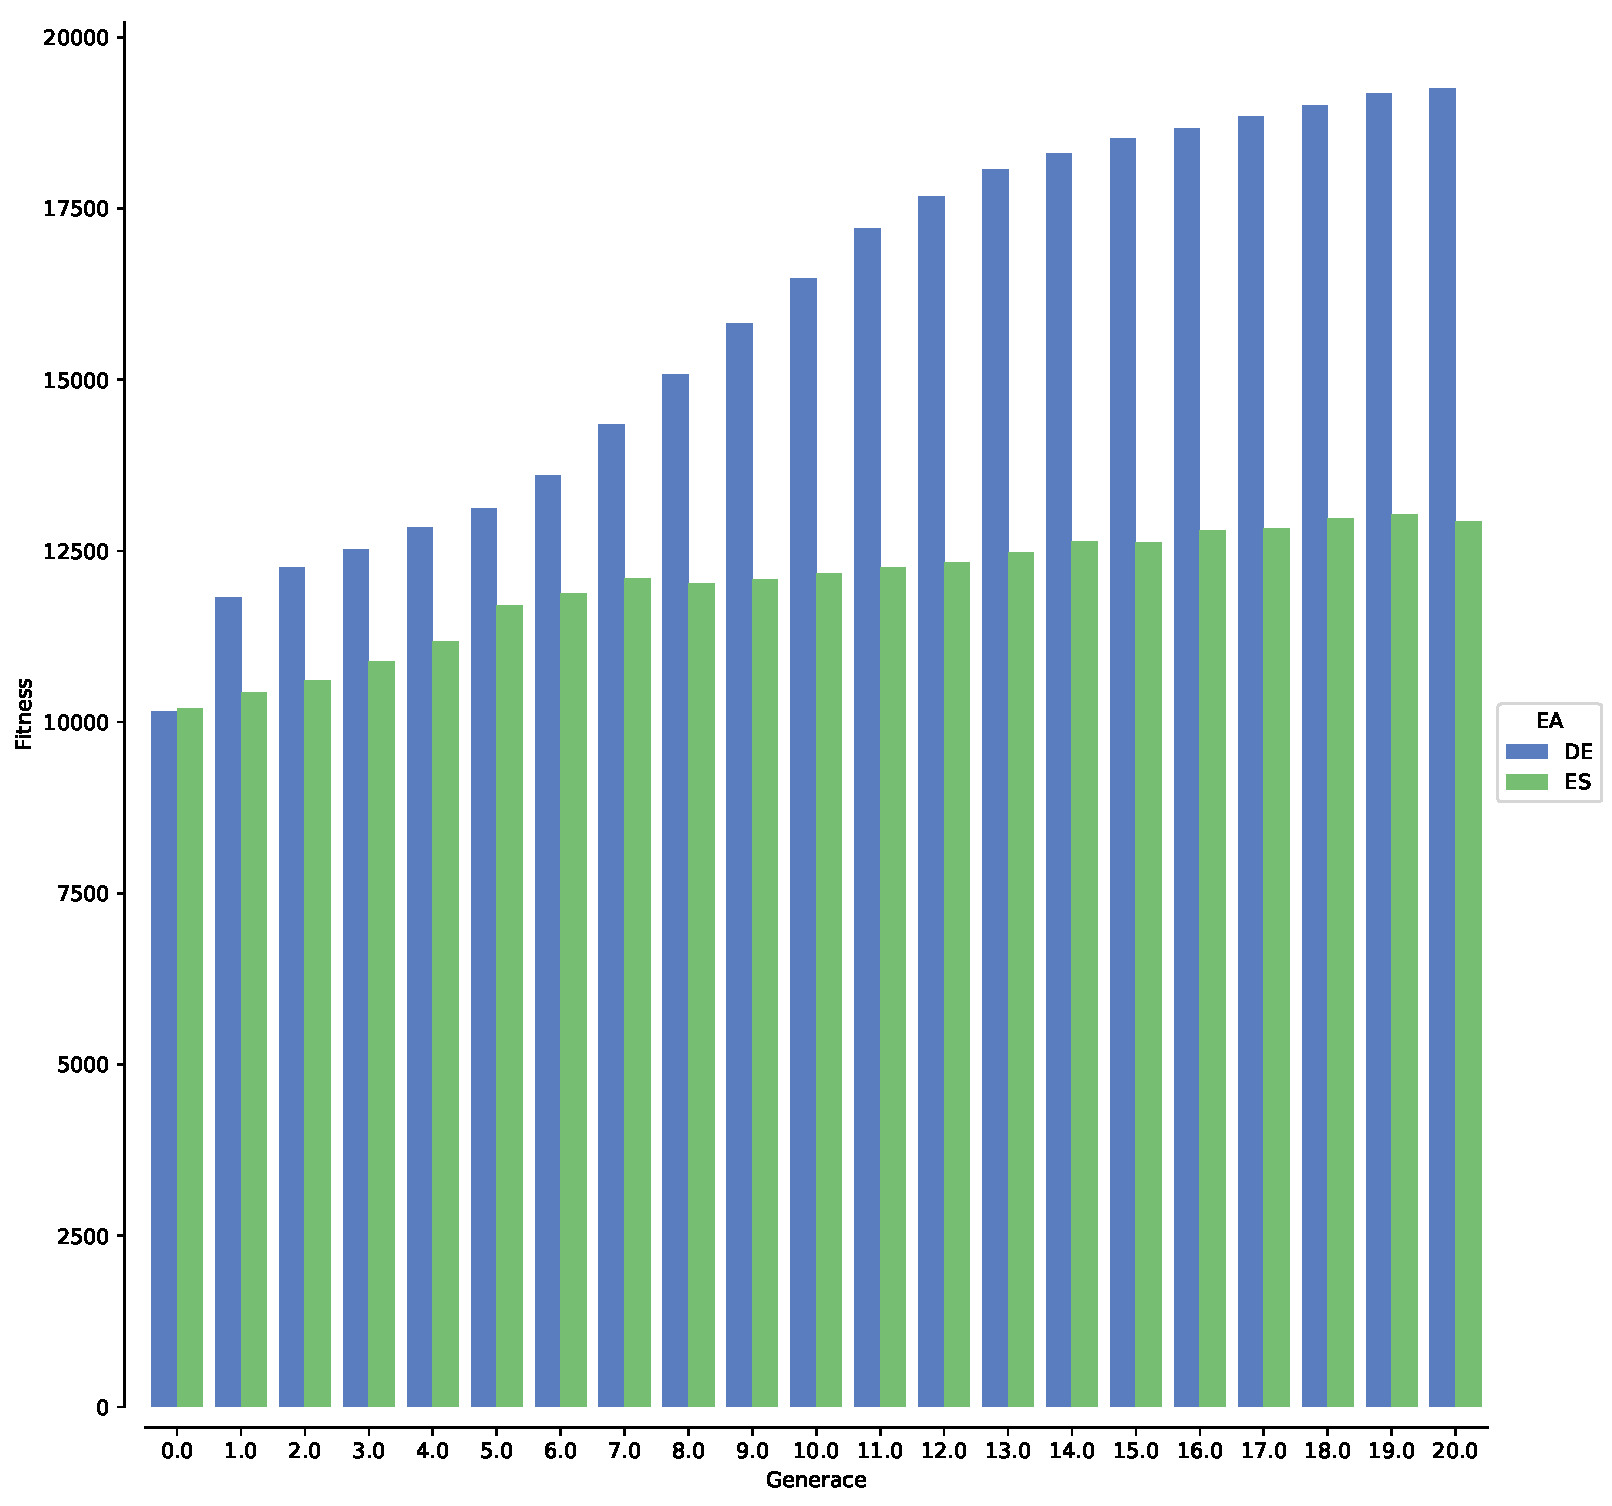
\includegraphics[width=\columnwidth]{../img/WoodMap/DEvsES/WorkerStockMem}
		\caption{Worker ukládání doprostřed  - porovnání průměrné fitness ES a DE}
		\label{obr04:StockESvsDE}
	\end{figure}


	\clearpage
	\subsubsection{Kooperace  hlavní úkol  - nastavení experimentu}
	V rámci posledního úkolu jsem složil už optimalizovaná chování dohromady, abych vytvořil heterogenní hejno řešící problém Wood Scene scénáře. Spojoval jsem náhodné chování pro Scout robota s náhodným u Worker robota, aby se našla nejlepší jejich kombinace, tak bylo nutné navýšit počet generací na 4000. Fitness funkce(\ref{tab04:Coop}) byla v tomto případě průnik posledních experimentů Worker ukládání doprostřed a Scout kácení. 
	\begin{table}[h]\centering   
		\begin{tabular}{l@{\hspace{1.5cm}}D{.}{,}{3.2}D{.}{,}{1.2}D{.}{,}{2.3}}
		\toprule
		\textbf{Nastavení mapy a EA}\\
		\midrule
			Roboti: & Scout-5, Worker-4 \\
			Počet generací: & 4000\\
			Počet iterací map & 2000\\
			Velikost generace(DE) & 200\\
			Počet jedinců(ES) & 10\\
			Počet mutovaný potomků(ES)&20\\
			Elitismus(ES)& Ano\\
			Elitismus(DE)& Ne \\
			\bottomrule
			\multicolumn{2}{l}{}
		\end{tabular}
		\par 
		\begin{tabular}{l@{\hspace{1.5cm}}D{.}{,}{3.2}D{.}{,}{1.2}D{.}{,}{2.3}}
			\toprule
			\textbf{Fitness funkce}\\
			\midrule
			Hodnota nalezeného pokáceného stromu &  100 \\
			Hodnota uloženého dřeva & 1000\\
			Hodnota dřeva v kontejneru & 100\\
			Hodnota jiné entity v kontejneru & -100\\
			Hodnota kolize & -1\\
			Ostatní hodnoty: & 0\\
			Počet stromů: & 400\\
			Počet už pokácených stromů & 0\\
			\bottomrule
			\multicolumn{2}{l}{}
		\end{tabular}
			\caption{Kooperace  hlavní úkol  - nastavení experimentu}
			\label{tab04:Coop}
	\end{table}

	Na \ref{obr04:CoopESvsDE} lze pozorovat, že pro ES bylo velmi obtížné skládat už úspěšné chování do lepších celků a velmi osciluje. ES uškodilo agresivní prohledávání prostoru a DE díky své architektuře vytěžilo z optimalizovaných chování maximum. Nejlepšímu jedinci se budeme věnovat podrobněji v další kapitole. 
		\clearpage
		\begin{figure}[t]\centering
		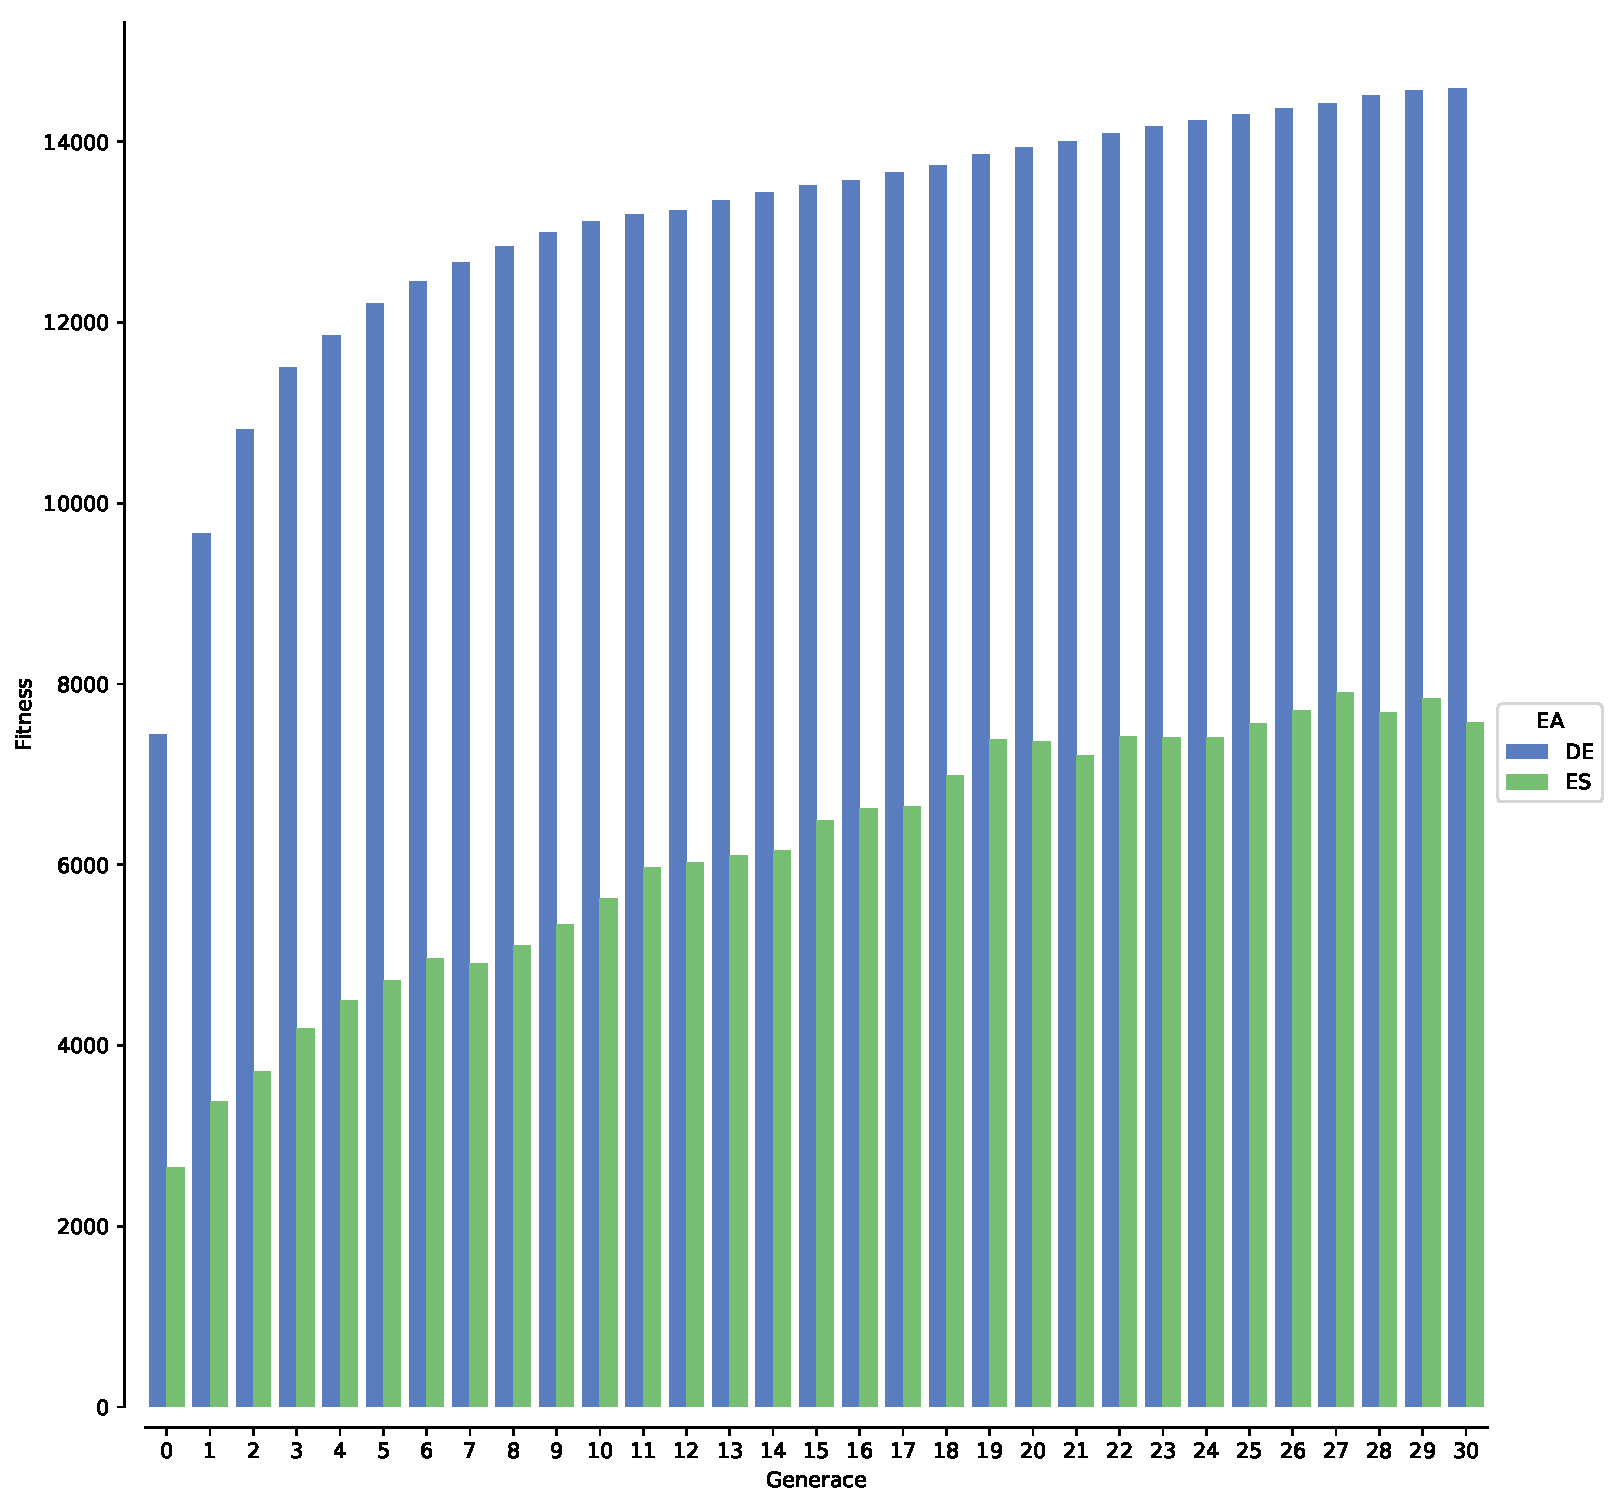
\includegraphics[width=\columnwidth]{../img/WoodMap/DEvsES/WoodCoopMem}
		\caption{Kooperace  hlavní úkol  - porovnání průměrné fitness ES a DE}
		\label{obr04:CoopESvsDE}
	\end{figure}
	\clearpage
	
	\subsection{Výsledky Experimentu}
	Výsledkem posloupnosti všech podúkolů vzniklo poměrně velmi komplexní chování. Finální neuronové sítě ať u Worker robotů, či Scout robotů se zvládají vyhýbat překážkám. Scout roboti kácí stromy, které naleznou. Worker roboti nakládají zpracované dřevo, pokud na něj narazí, když zachytí signál úložiště, tak vyloží aktuální náklad. Některá chování byla také schopna předejít zaseknutí o nějaký shluk objektů, pokud byl  jejich pohyb vpřed neúspěšný, tak po několika pokusech roboti vycouvali a vydali se cestou okolo kritického místa. U většiny se také objevilo použití rádiových signálů jako prostředku pro největší možné rozptýlení po mapě, jakmile zachytí cizí signál vydají se opačným směrem. Průběh fitness jednotlivých podúkolů je zachycena na předchozích grafech \ref{obr04:Walk} až \ref{obr04:StockES}. V tabulce \ref{tab04:WoodStat} můžete vyčíst průměrné počty nalezených stromů, uskladněného materiálu, apod ze 100 simulací mapy. 
	
	Ač se jedná o nejlepší dosažené chování objevují se nějaké nedostatky. Worker robot se občas dostane do pozice, ze které není schopen vyjet, jedná se především o kolize s vícero entitami. Tento problém by mohlo vyřešit použití vícevrstvých sítí či evolučního algoritmu evolvujícího i architekturu sítě. Skládání zpracovaného materiálu po obvodu skladiště není efektivní způsob, jak do něj naskládat maximální množství dřeva. V tomto případě jsem se snažil vylepšit tento nedostatek promítnutím vzdálenosti dřeva od středu skladiště do celkové fitness, ovšem bez znatelného zlepšení v chování. Nejspíše by bylo třeba použít rádiový senzor poskytující více informací o směru k zachycenému signálu. 
	
		\begin{table}[h]\centering   
		\begin{tabular}{l@{\hspace{1.5cm}}D{.}{,}{3.2}D{.}{,}{1.2}D{.}{,}{2.3}}
			\toprule
			& \mc{} & \mc{}\\
		\textbf{Inicializační nastavení:}  \\
			\midrule
			Výška & 800\\ 
			Šířka & 1200\\
			Počet iterací & 10000\\
			Počet stromů & 400\\
			Počet Scout robotů & 5\\
			Počet Worker robotů & 4\\
			\bottomrule
			\multicolumn{2}{l}{}
		\end{tabular}
		\caption{WoodScene - nastavení mapy pro testovací experiment}
	\end{table}
	\begin{table}[h]\centering   
		\begin{tabular}{l@{\hspace{1.5cm}}D{.}{,}{3.2}D{.}{,}{1.2}D{.}{,}{2.3}}
			\toprule
			& \mc{} & \mc{}\\
			\textbf{Výsledky} \\
			\bottomrule
			Zpracované dřevo zanechané v mapě & 225.22\\
			Stromy v mapě & 156.22\\
			Z toho nalezené & 52.84\\
			Dřevo v kontejnerech & 18.48\\
			Uskladněné dřevo & 17.56\\
			\multicolumn{2}{l}{}
		\end{tabular}
		\caption{WoodScene - výsledky simulace nejlepšího jedince, průměr ze 100 simulací testovacího experimentu}
		\label{tab04:WoodStat}
	\end{table}
	\newpage 
	\begin{figure}[p]\centering
		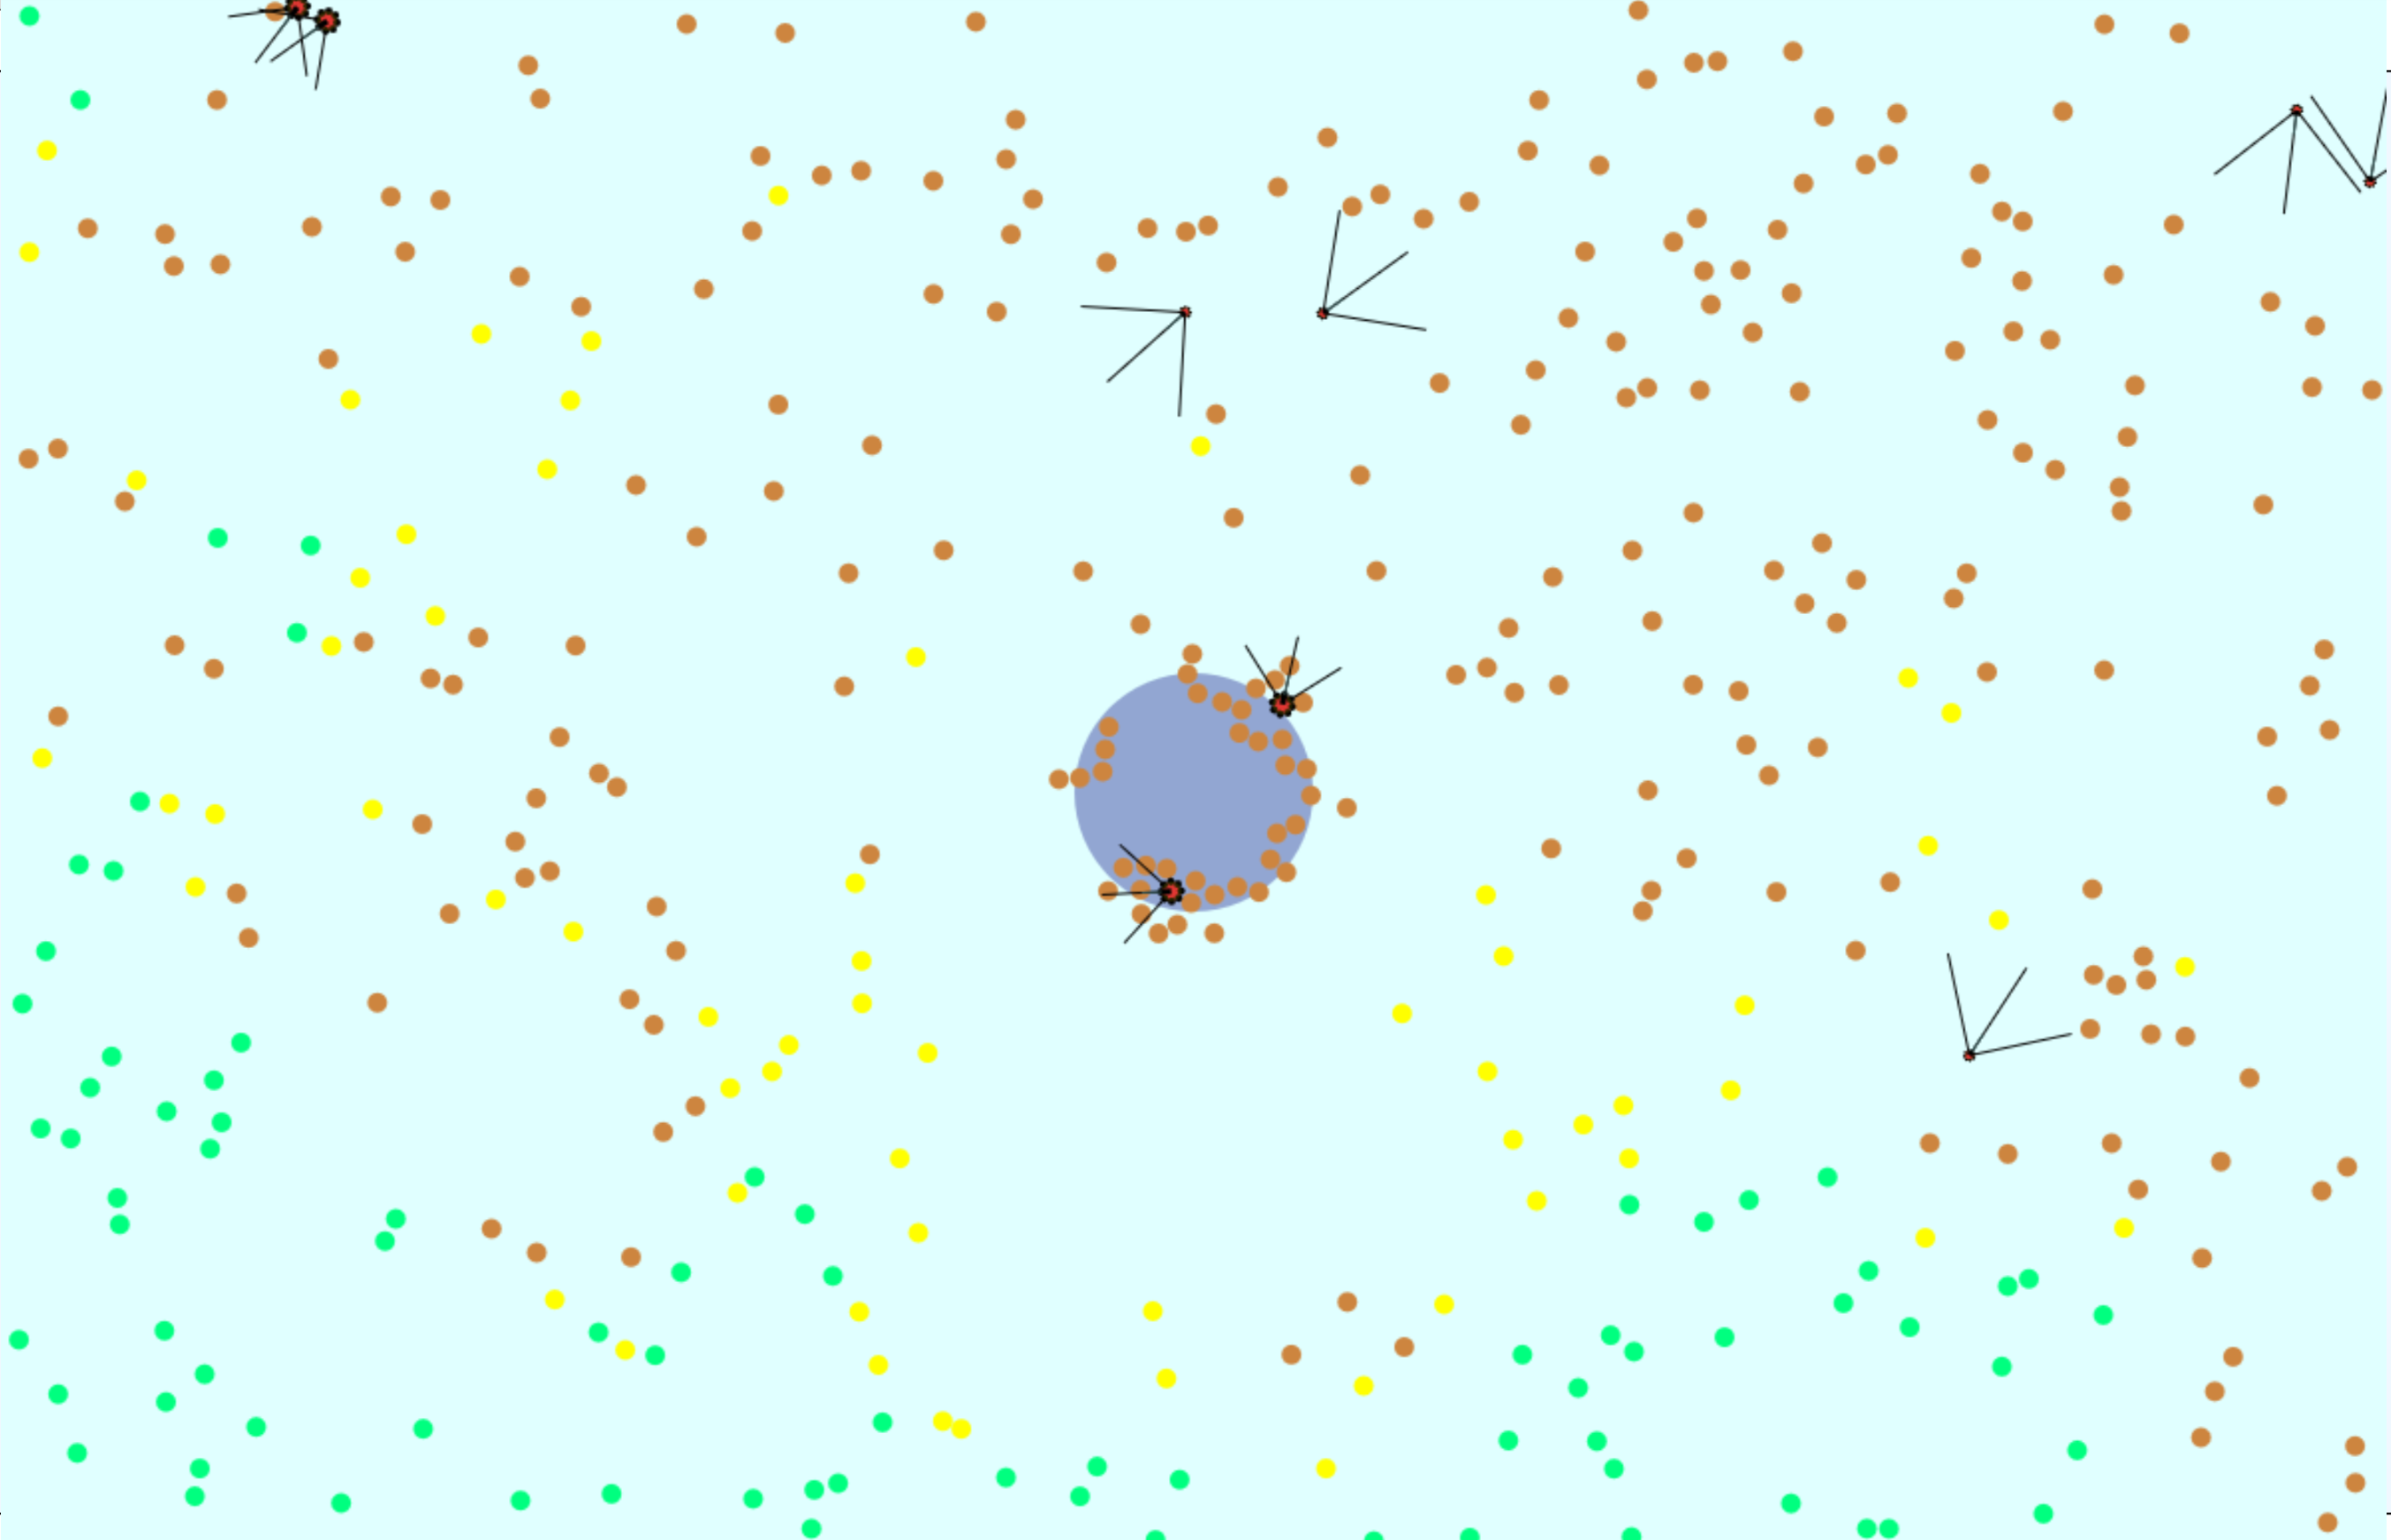
\includegraphics[width=\columnwidth]{../img/WoodMap/pictures/end.png}
		\caption{Nejlepší jedinec - 10000 iterací simulace}
		\label{obr04:bestEnd}
	\end{figure}
	\begin{figure}[p]\centering
		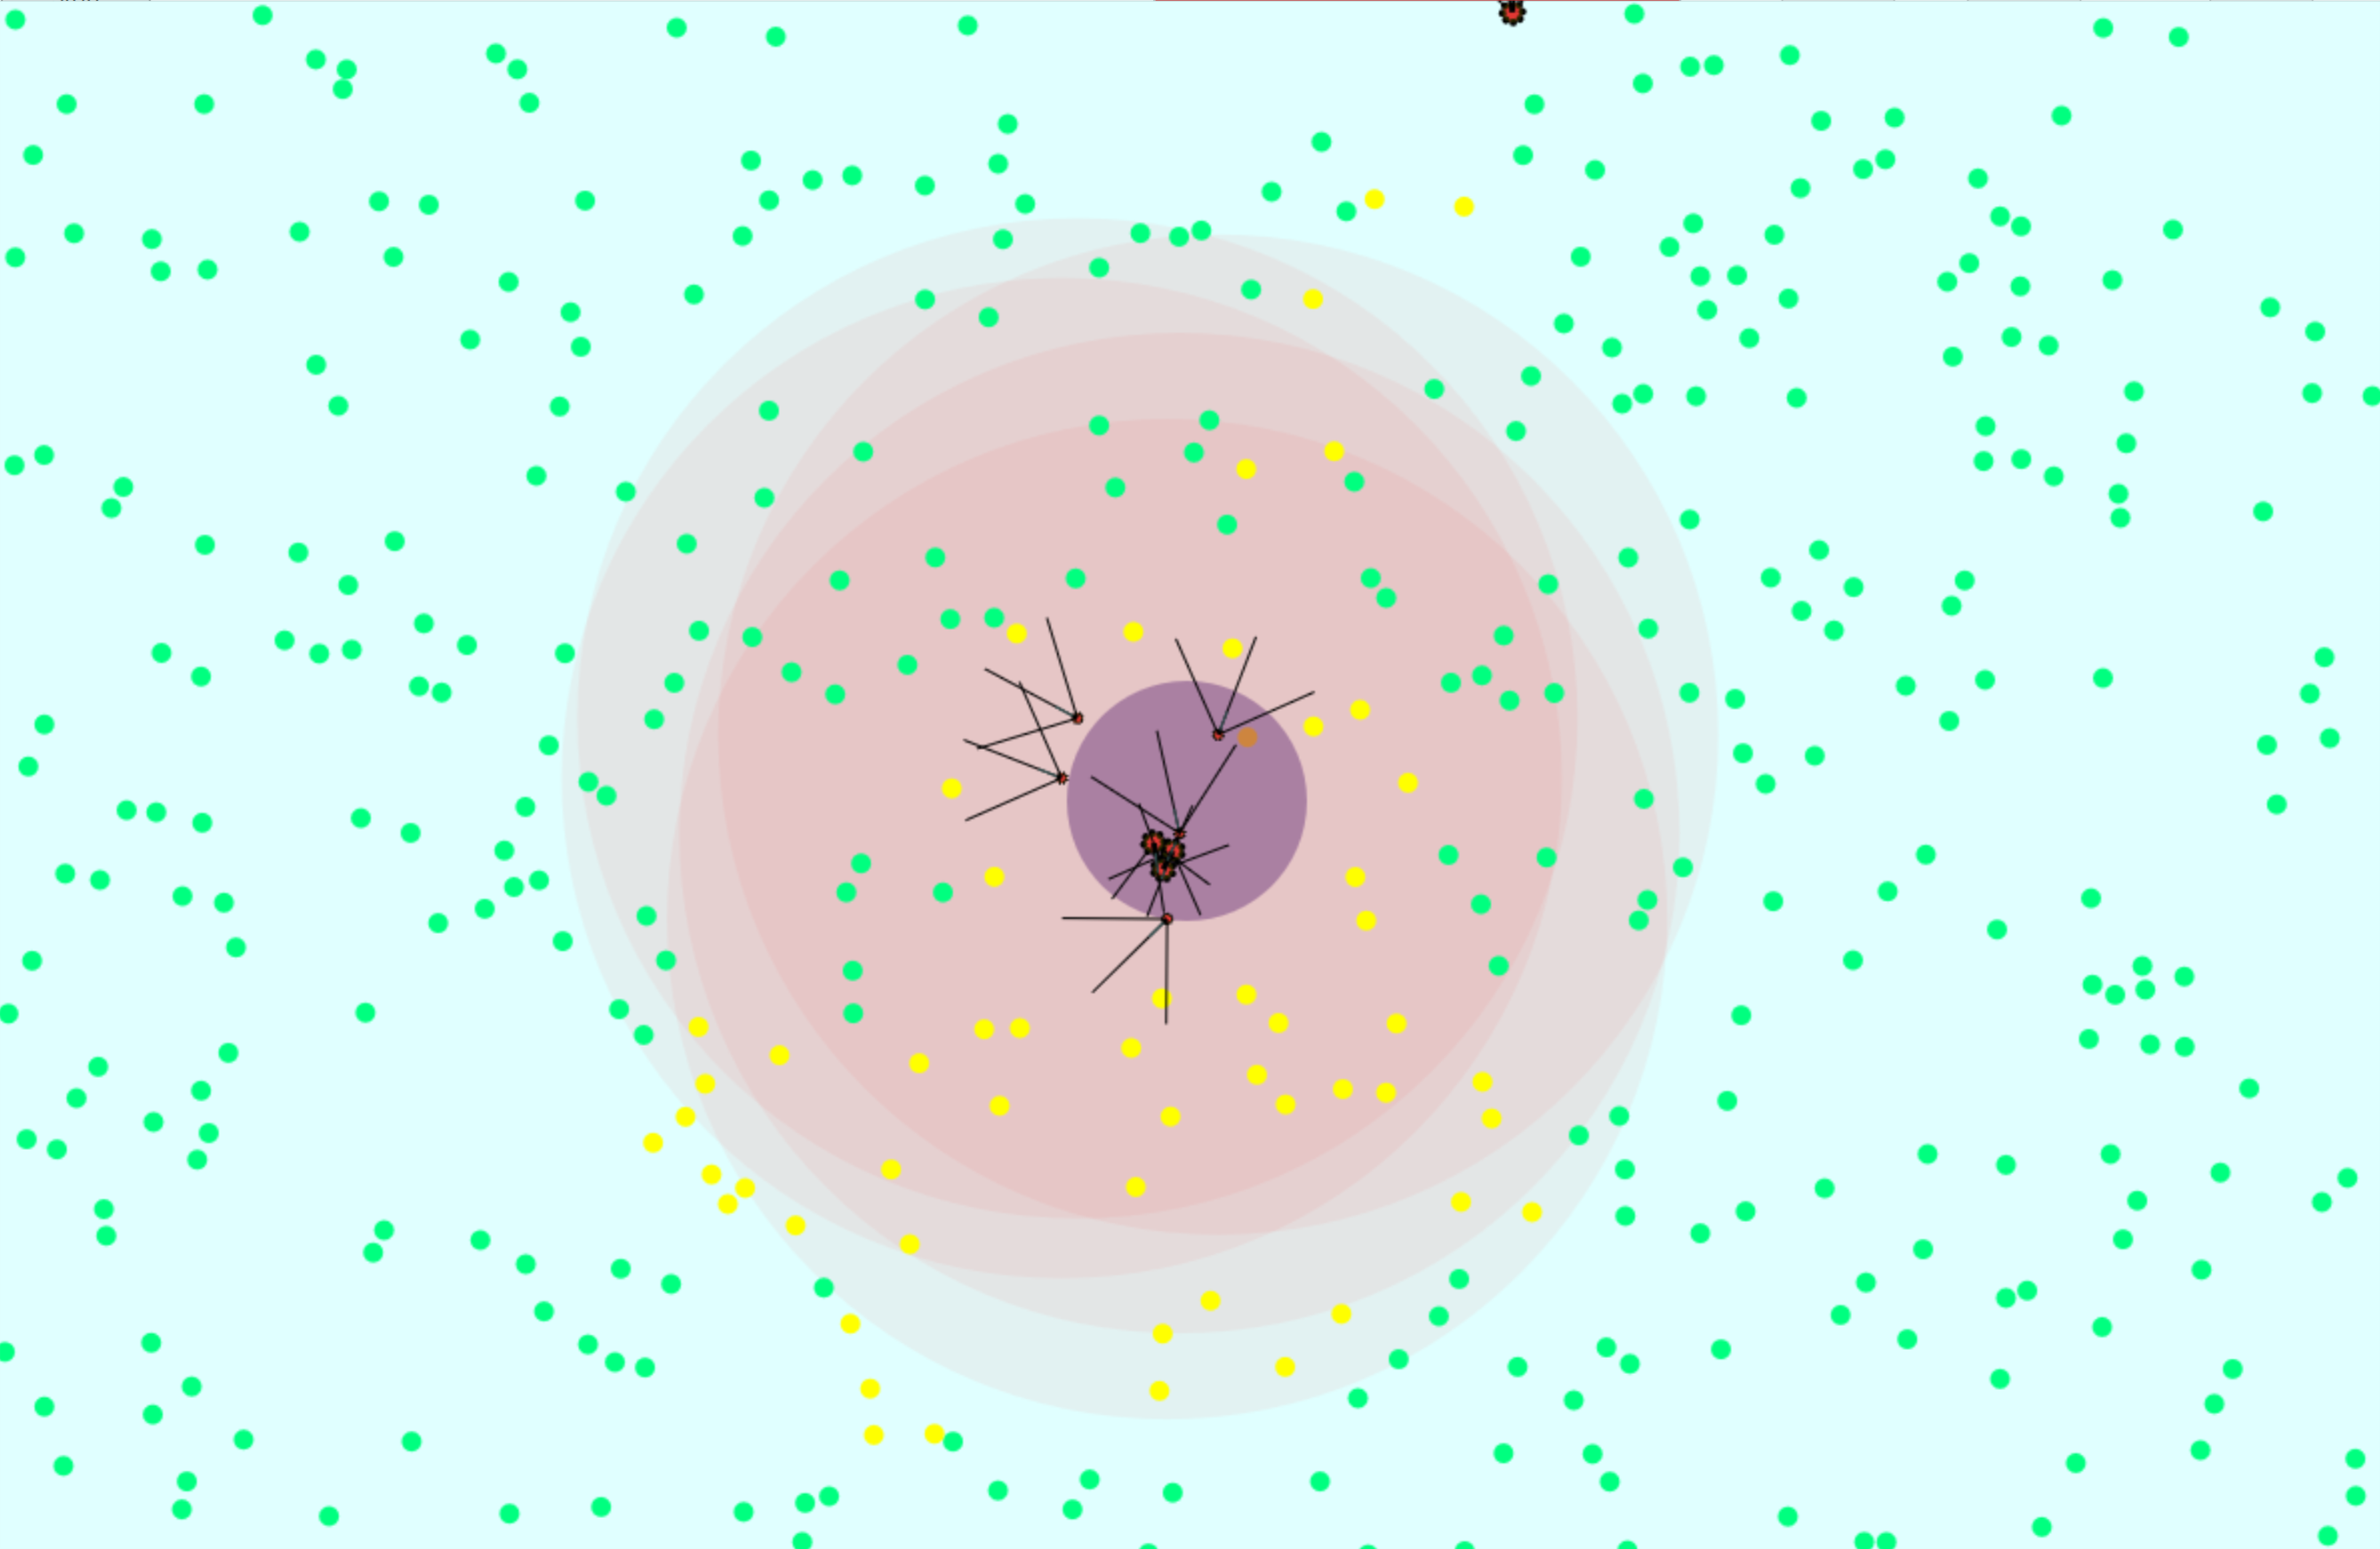
\includegraphics[width=\columnwidth]{../img/WoodMap/pictures/EndRandom.png}
		\caption{Náhodný jedinec - 10000 iterací simulace}
		\label{obr04:randomEnd}
	\end{figure}
	\clearpage
\section{Mineral Scene}
Tento scénář si bere jako inspiraci strategické hry např. Starcraft \citep*{starcraft} a hypotetické přežití robotů na cizí planetě, kde si budou muset obstarat vlastní nerostné suroviny pro běh. Opět je klíčová spolupráce mezi roboty, kdy roboti mají odlišné určení. Jejich společným cílem je maximalizovat množství vyrobeného paliva.
\par 
V mém zjednodušeném scénáři se palivo se vyrábí z minerálů, které jsou náhodně rozmístěny po mapě. Transformaci minerálu na palivo dokáže pouze největší robot Refactor. V mapě se dále nacházejí překážky a volné palivo, které mohou roboti ihned po sebrání použít. V rámci hlavního cíle roboti musí nejdříve nalézt minerál, Refactor jej přeměnit a pak případně předat ostatním robotům. \unsure{Je to hodně komplexní asi to zjednoduším}
\par
V Mineral Scene figurují dohromady 3 rozliční roboti, všichni potřebují pro pohyb odlišné množství paliva. Nejmenší robot (Mineral Scout) disponuje pouze senzory k exploraci prostředí a rádiovým vysílačem pro komunikaci se skupinou, opět má unikátní kód  jako v předchozím scénáři. Robot střední velikosti (Mineral Worker) se pohybuje o něco pomaleji než Mineral Scout, ale umí přesouvat objekty i více najednou. Robot pro přeměnu minerálu (suroviny na výrobu paliva) označen v simulaci jako Mineral Refactor se přemisťuje nejpomaleji, má možnost přeměnit minerál na palivo. 
\par
Jedná se o složitější cíl než v předchozím scénáři. V mapě se vyskytují navíc překážky a celkový počet entit na mapě je vyšší. Zatímco ve Wood Scene je místo pevně místo přesunu surovin pěkně dané, zde se musí transportní roboti hledat Refaktor roboty. Tento scénář jsem navrhl hlavně k nalezení limitou mnou navržené metody. 
\par 
Na obrázku \ref{obr04:MineralSceneRandomStart} je vyobrazena vizualizace daného scénáře. Roboti jsou vybarveni červenou barvou a jednotlivé druhý od sebe lze snadno rozeznat podle velikosti (nejmenší Scout robot, poté Worker robot a největší Refaktor robot), Zelené kroužky představují minerály, pokud je minerál objevený hejnem obarví se žlutě. Šedivou barvou jsou vyvedeny překážky a palivo černou.
\clearpage

\begin{figure}[p]\centering
	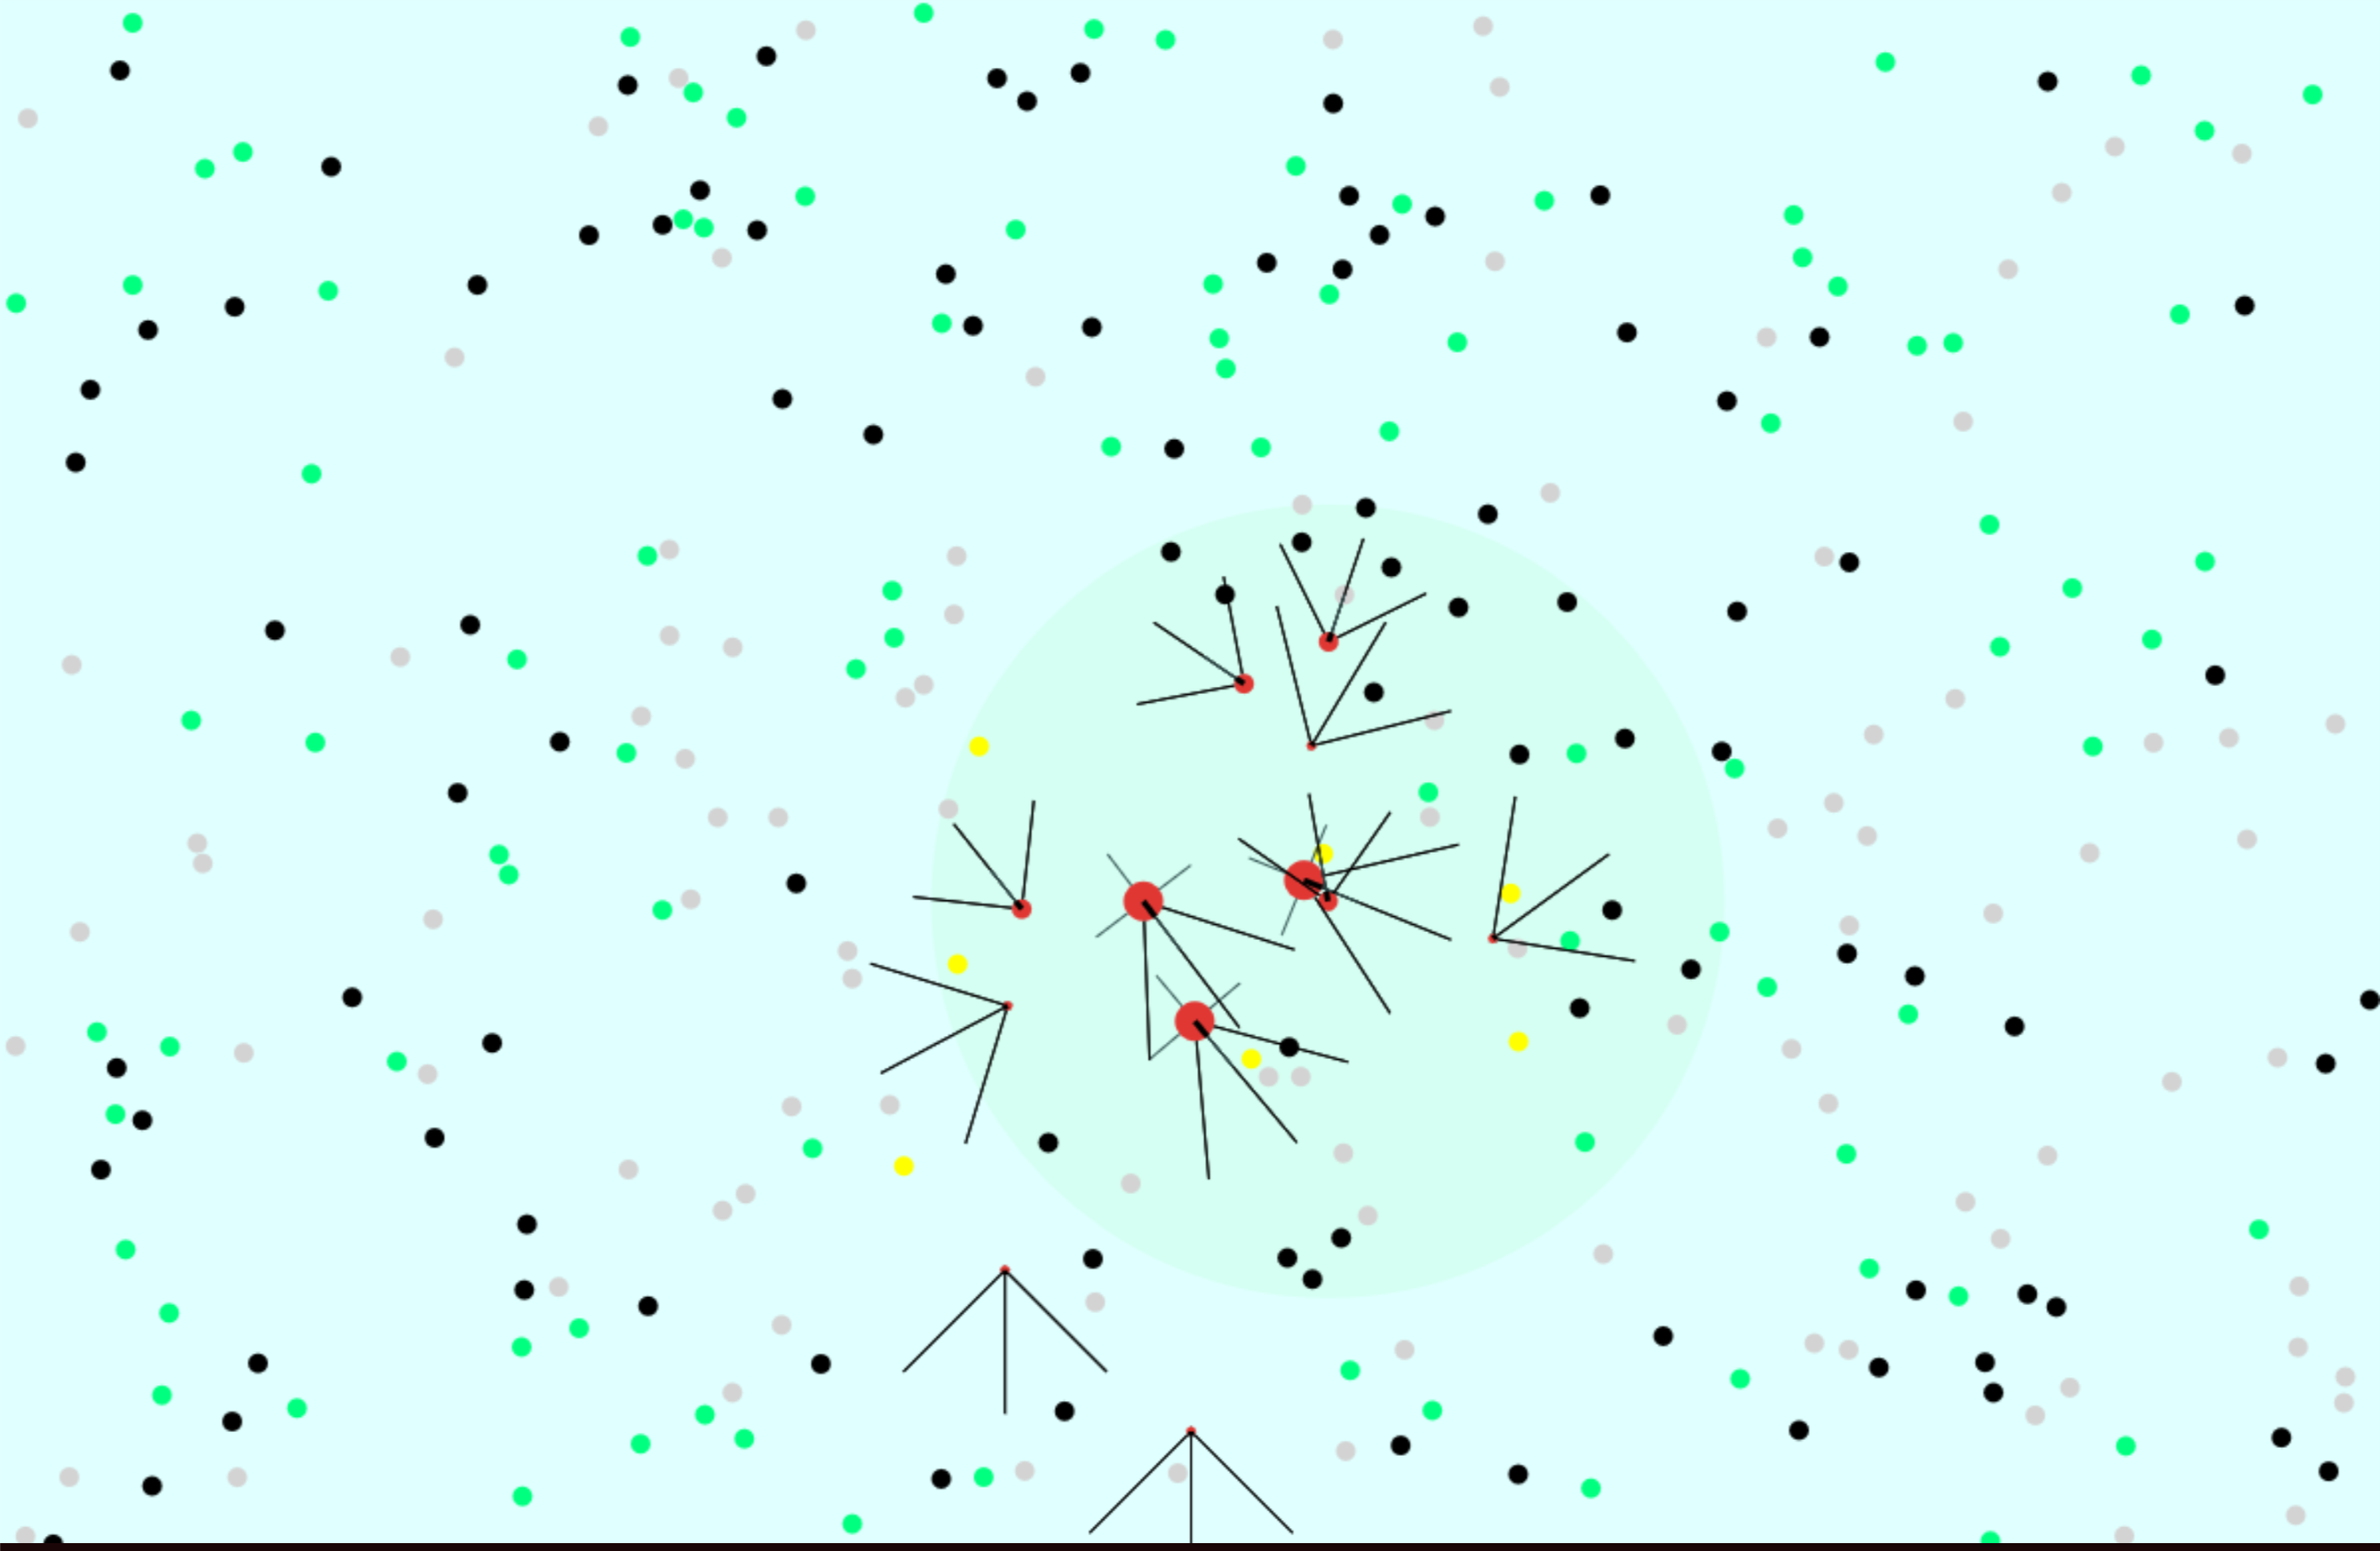
\includegraphics[width=\columnwidth]{../img/MineralMap/MineralRandom.png}
	\caption{Příklad Mineral Scene mapy: start náhodného chování}
	\label{obr04:MineralSceneRandomStart}
\end{figure}
\clearpage 
\subsection{Roboti}
V Mineral Scene scénáři se vyskytuje 12 robotů. V hejnu se vyskytují 3 různé druhy robotů: Scout roboti, Worker roboti, Refaktor roboti. V implementaci jsou odlišeni od předchozího experimentu prefixem Mineral. Jejich ovládání stejně jako v předchozím experimentu probíhá pomocí neuronových sítí. Jedinec má opět podobu vektoru vah jednotlivých neuronových sítí a hodnoceno je komplet celé hejno. Každý robot má nádrž na palivo a každá iterace mapy ho stojí jednu jednotka paliva. Popišme jednotlivé roboty.
\subsubsection{Scout robot}
Jak název napovídá Scout robot prozkoumává mapu. Oproti Wood Scene nemá žádnou další funkci. Ze všech robotů se pohybuje nejrychleji a díky malé velikosti dokáže projíždět i užšími prostory. Informace o prostředí získává pomocí úsečkových senzorů a velkého kruhového senzoru, který poskytuje počet jednotlivých druhů entit v celém okruhu. Pro komunikaci se zbytkem používá rádiový signál s kódem 0. 
\par  

\begin{table}[h]\centering
	\begin{tabular}{l@{\hspace{1.0cm}}D{.}{,}{2.2}D{.}{,}{2.2}D{.}{,}{2.3}}
		\toprule
		\textbf{Scout Robot} \\
		\midrule
		Tvar: & Kruh\\
		Poloměr: & 2,5\\
		Namespace: & MineralRobots\\
		Název: & ScoutRobotMem \\
		Velikost kontejneru: & 0\\
		\midrule
		\textbf{Efektory} \\
		\midrule
		Motor: & Dvou kolečkový \\
		Maximální rychlost: & 3 \\
		Kód rádiového signálu: & 0\\
		Poloměr signálu: & 200\\
		Počet paměťových slotů: &10 \\
		Obsah slotu: & float\\
		\midrule
		\textbf{Senzory} \\
		\midrule
		Počet line senzorů: &  3\\
		Délka line senzorů: & 70\\
		Orientace l. senzorů: & 0^\circ, 45^\circ, -45^\circ\\
		Počet fuel senzorů: &  3\\
		Délka fuel senzorů: & 70\\
		Orientace f. senzorů: & 0^\circ, 45^\circ, -45^\circ\\
		Poloměr rádiového přijímače: & 100 \\
		Počet touch senzorů: & 3 \\  
		Lokátorový senzor\\ 
		\bottomrule
		\multicolumn{2}{l}{}
	\end{tabular}
	\caption{Mineral Scene - Scout robot popis }
	\label{tab04:MineralScout}
\end{table}
\clearpage
\subsubsection{Worker Robot}
Mineral Worker roboti zastupují úlohu transportu minerálů. Pohybují se rychleji než Refaktor roboti, ale zase pomaleji než Scout roboti. Uloží do svého kontejneru až 5 minerálů. Pro komunikaci využívají rádiového signálu s kódem 1. Samozřejmě má k dispozici Picker pro nákládání a vykládání entit z kontejneru.
\begin{table}[h]\centering
	\begin{tabular}{l@{\hspace{1.0cm}}D{.}{,}{2.2}D{.}{,}{2.2}D{.}{,}{2.3}}
		\toprule
		\textbf{Worker Robot} \\
		\midrule
		Tvar: & Kruh\\
		Poloměr: & 5 \\
		Namespace: & MineralRobots\\
		Název: & WorkerRobotMem \\
		Velikost kontejneru: & 5\\
		\midrule
		\textbf{Efektory} \\
		\midrule
		Motor: & Dvou kolečkový \\
		Maximální rychlost: & 1,5 \\
		Kód rádiového signálu: & 1\\
		Poloměr signálu: & 200\\
		Dosah pickeru: & 10\\
		Počet paměťových slotů: &10 \\
		Obsah slotu: & float\\
		\midrule 
		\textbf{Senzory} \\
		\midrule
		Počet line senzorů: &  3\\
		Délka line senzorů: & 50\\
		Orientace l. senzorů: & 0^\circ, 45^\circ, -45^\circ\\
		Počet fuel senzorů: &  3\\
		Délka fuel senzorů: & 50\\
		Orientace f. senzorů: & 0^\circ, 45^\circ, -45^\circ\\
		Poloměr rádiového přijímače: & 100 \\
		Počet touch senzorů: & 3 \\  
		Lokátorový senzor\\ 
		\bottomrule
		\multicolumn{2}{l}{}
	\end{tabular}
	\caption{Mineral Scene - Worker robot popis }
	\label{tab04:MineralWorker}
\end{table}
\clearpage
\subsubsection{Refaktor robot}
Nenahraditelnou roli zastává Mineral Scene, dokáže totiž měnit minerál na jednotku paliva. Pro přeměnu musí být minerál připraven na vrcholu kontejneru a po procesu přeměny se místo minerálu objeví palivo. Refaktor robot je však oproti ostatním robotů značně neohrabaný, zvláště kvůli jeho velikosti, jeho poloměr odpovídá dvěma Worker robotům (resp. čtyřem Scout robotům). Pohybuje se z nich také nejpomaleji. Jeho rádiové signály nesou kód 2. Nakladače (vykladače) má do všech čtyrech světových směrů. 
\par  
\begin{table}[h]\centering
	\begin{tabular}{l@{\hspace{1.0cm}}D{.}{,}{2.2}D{.}{,}{2.2}D{.}{,}{2.3}}
		\toprule
		\textbf{Refaktor Robot} \\
		\midrule
		Tvar: & Kruh\\
		Poloměr: & 10 \\
		Namespace: & MineralRobots\\
		Název: & RefactorRobotMem \\
		Velikost kontejneru: & 5\\
		\midrule
		\textbf{Efektory} \\
		\midrule
		Motor: & Dvou kolečkový \\
		Maximální rychlost: & 1,5 \\
		Kód rádiového signálu: & 2\\
		Poloměr signálu: & 200\\
		Počet pickerů & 4\\
		Orientace pickerů & po\ 90^\circ\\ 
		Dosah pickerů: & 20\\
		Počet paměťových slotů: &10 \\
		Obsah slotu: & float\\
		Refaktor: & Minerál \Rightarrow Palivo \\
		Dosah refaktoru:  & kontejner \\
		Kapacita refaktoru: & 1\\ 
		\midrule 
		\textbf{Senzory} \\
		\midrule
		Počet line senzorů: &  3\\
		Délka line senzorů: & 70\\
		Orientace l. senzorů: & 0^\circ, 35^\circ, -35^\circ\\
		Počet fuel senzorů: &  3\\
		Délka fuel senzorů: & 70\\
		Orientace f. senzorů: & 0^\circ, 35^\circ, -35^\circ\\
		Poloměr rádiového přijímače: & 100 \\
		Počet touch senzorů: & 3 \\  
		Lokátorový senzor\\ 
		\bottomrule
		\multicolumn{2}{l}{}
	\end{tabular}
	\caption{Mineral Scene - Refaktor robot popis }
	\label{tab04:MineralRefactor}
\end{table}
\clearpage
\subsection{Vyhodnocování Fitness}
Fitness funkce pro Mineral Scene scénář jsem, po dobrých zkušenostech z předchozího experimentu, použil vážený součet následujících charakteristik mapy po konci simulace. Tento součet je specifický pro každý podúkol zvlášť. Kvůli komplexnosti toho úkolu a velikosti hejna v jednotlivých podúkolech nevystupují roboti vždy v plném počtu, ale nejdříve se optimalizuje chování pro pár jedinců od každého druhu. I tak bylo potřeba zmenšit velikost populace pro rozumnou dobu času běhu. Pozitivní hodnocení roboti získávali za: 
\begin{itemize}
	\item \textit{objevené minerály} - minerály o které zavadil line senzor
	\item \textit{uložené minerály} - minerály nacházející se v kontejnerech robotů 
	\item \textit{přeměněné palivo} - palivo nacházející se na mapě či v kontejnerech robotů
	\item \textit{palivo v nádržích} - palivo uvnitř nádrží jednotlivých robotů
	\item \textit{odložené minerály} - minerály na pomocném prostoru označeným rádiovým signálem
\end{itemize}
A negativní pouze za: 
\begin{itemize}
	\item \textit{kolize} - počet pokusů o pohyb který by vedl ke kolizi
\end{itemize}
\subsection{Podúkoly}
Podle výsledků předchozího experimentu jsem se tentokrát výhradně soustředil na DE, které vycházelo v celkovém důsledku jako lepší. \unsure{Nevím, zda to stihnu} 
\par 
Opět jsem vygeneroval první neuronové sítě náhodně i další kroky jsou podobné jako v předchozím případě, nejdříve jsem navrhl fitness funkce pro učení chůze, vyhýbání, sbírání objektů a jejich skládání. Dále jsem však nebyla zřejmá posloupnost jednotlivých úkonů, proto fitness funkce odpovídá už výslednému cíli, množství vytvořeného paliva a sebraným minerálů.
\par 
Dále budou následovat konkrétní metaúkoly. U každého metaúkolu bude uveden krátký popis cíle jednotlivého experimentu, obrázek s grafy průběhem fitness, stručné shrnutí chování a grafů s průběhy. Grafy budou vždy stejného formátu,  y osa zobrazuje hodnotu fitness, x osa odpovídá číslu generace, pro lepší čitelnost jsou generace sdruženy po 10. 
\clearpage

\subsubsection{Scout chůze - nastavení experimentu}
Stejně jako u předchozího scénáře, jsem roboty nejdříve učil pohybu. Opět jsem roboty oddělil, aby optimalizace neupřednostňovala ty rychlejší. Náhodně vygenerované neuronové sítě pro řízení Scout robotů. Poté jsou optimalizovány pomocí fitness, která oceňuje chování podle počtu objevených minerálů.
\begin{table}[h]\centering   
	\begin{tabular}{l@{\hspace{1.5cm}}D{.}{,}{3.2}D{.}{,}{1.2}D{.}{,}{2.3}}
		\toprule
		\textbf{Nastavení mapy a EA}\\
		\midrule
		Roboti: & Scout-5 \\
		Počet generací: & 1000\\
		Počet iterací map & 1000\\
		Velikost generace(DE) & 100\\
		\bottomrule
		\multicolumn{2}{l}{}
	\end{tabular}
	\par 
	\begin{tabular}{l@{\hspace{1.5cm}}D{.}{,}{3.2}D{.}{,}{1.2}D{.}{,}{2.3}}
		\toprule
		\textbf{Fitness funkce}\\
		\midrule
		Hodnota nalezeného minerálu &  100 \\
		Ostatní hodnoty: & 0\\
		Počet minerálů: & 400\\
		Počet překážek & 100\\
		Počet paliva & 100\\
		\bottomrule
		\multicolumn{2}{l}{}
	\end{tabular}
	\caption{Scout chůze - nastavení experimentu}
	\label{tab04:MineralScoutWalk}
\end{table}
Z grafu \ref{obr04:MineralScoutWalk} lze vyčíst, že ani větší množství entit v mapě nevadilo pro optimalizaci slušného chování pro vyhýbání se překážkám a prohledávání mapy. Nejlepší chování dokáže odhalit okolo 75\% minerálů na mapě.
\clearpage
\begin{figure}[t]\centering
	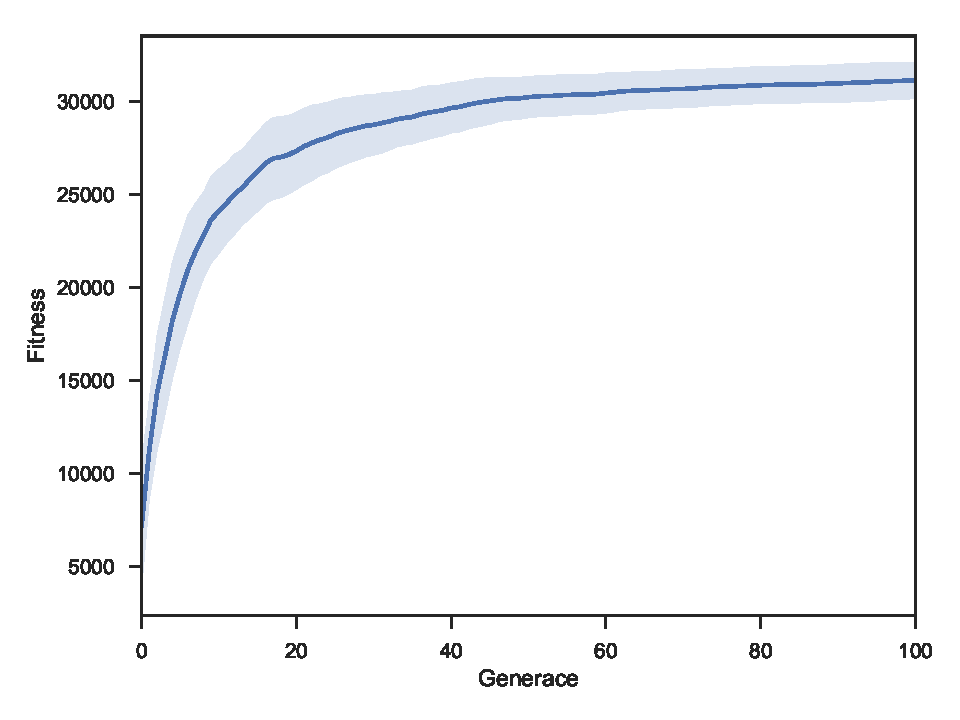
\includegraphics[width=\columnwidth]{../img/MineralMap/MineralScoutWalk}
	\caption{Mineral Scout chůze -  průběh fitness DE}
	\label{obr04:MineralScoutWalk}
\end{figure}
\clearpage

\subsubsection{Worker chůze - nastavení experimentu}
I pro Worker robota bylo potřeba optimalizovat chůzí v mapě. Stejně jako Scout robot byli odměňovány za nalezené Minerály. 
\par
\begin{table}[h]\centering   
	\begin{tabular}{l@{\hspace{1.5cm}}D{.}{,}{3.2}D{.}{,}{1.2}D{.}{,}{2.3}}
		\toprule
		\textbf{Nastavení mapy a EA}\\
		\midrule
		Roboti: & Worker-4 \\
		Počet generací: & 1000\\
		Počet iterací map & 1000\\
		Velikost generace(DE) & 100\\
		\bottomrule
		\multicolumn{2}{l}{}
	\end{tabular}
	\par 
	\begin{tabular}{l@{\hspace{1.5cm}}D{.}{,}{3.2}D{.}{,}{1.2}D{.}{,}{2.3}}
		\toprule
		\textbf{Fitness funkce}\\
		\midrule
		Hodnota nalezeného minerálu &  100 \\
		Ostatní hodnoty: & 0\\
		Počet minerálů: & 300\\
		Počet překážek & 100\\
		Počet paliva & 100\\
		\bottomrule
		\multicolumn{2}{l}{}
	\end{tabular}
	\caption{Mineral Worker chůze - nastavení experimentu}
	\label{tab04:MineralWorkerWalk}
\end{table}
Nejlepší chování u Worker robota dokáže objevit více než čtvrtinu minerálů, jak ukazuje obrázek \ref{obr04:MineralWorkerWalk} Což je také uspokojivý výsledek, přihlédneme-li k tomu, že Scout robot má poloviční rychlost a velikost než Worker robota, navíc má kratší line senzory. 
\clearpage
\begin{figure}[t]\centering
	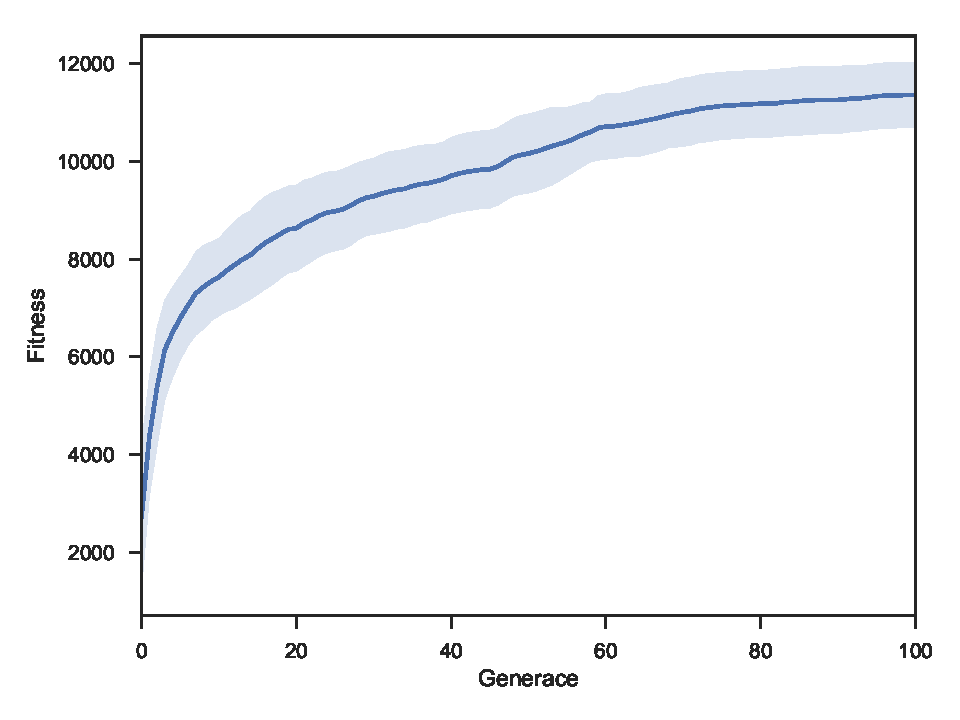
\includegraphics[width=\columnwidth]{../img/MineralMap/MineralWorkerWalk}
	\caption{Mineral Worker chůze -  průběh fitness DE}
	\label{obr04:MineralWorkerWalk}
\end{figure}
\clearpage

\subsubsection{Worker sbírání - nastavení experimentu}
Stejně jako ve Wood Scene bylo klíčové sbírání už zpracováného dřeva, tak v Mineral Scene jsem cílil na maximální počet sebraného paliva. Na rozdíl od Wood Scene však není zcela jasné, kam ukládat sebrané minerály. Aby v budoucích podúkolech umisťovali roboti, co nejblíže k Refaktor robotům, přidal jsem proto prozatímně do středu mapy pomocný rádiový signál se stejným kódem jako mají Refaktor roboti. 
\par
\begin{table}[h]\centering   
	\begin{tabular}{l@{\hspace{1.5cm}}D{.}{,}{3.2}D{.}{,}{1.2}D{.}{,}{2.3}}
		\toprule
		\textbf{Nastavení mapy a EA}\\
		\midrule
		Roboti: & Worker-2 \\
		Počet generací: & 3000\\
		Počet iterací map & 1000\\
		Velikost generace(DE) & 100\\
		\bottomrule
		\multicolumn{2}{l}{}
	\end{tabular}
	\par 
	\begin{tabular}{l@{\hspace{1.5cm}}D{.}{,}{3.2}D{.}{,}{1.2}D{.}{,}{2.3}}
		\toprule
		\textbf{Fitness funkce}\\
		\midrule
		Pomocný rádiový signál: & Ano\\
		Hodnota nalezeného minerálu &  1\\
		Hodnota minerálu v pomoc. signálu & 1010\\ 
		Hodnota uložených minerálů & 1000\\
		Ostatní hodnoty: & 0\\
		Počet minerálů: & 400\\
		Počet překážek & 100\\
		Počet paliva & 100\\
		\bottomrule
		\multicolumn{2}{l}{}
	\end{tabular}
	\caption{Mineral Worker sbírání - nastavení experimentu}
	\label{tab04:MineralWorkerPickUp}
\end{table}
Roboti v prvních 500 generacích zaplní své kontejnery minerály, což může pozorovat na  grafu \ref{obr04:MineralWorkerPickUp}. Dále dokonce dováželi roboti do středu několik minerálů. 
\begin{figure}[t]\centering
	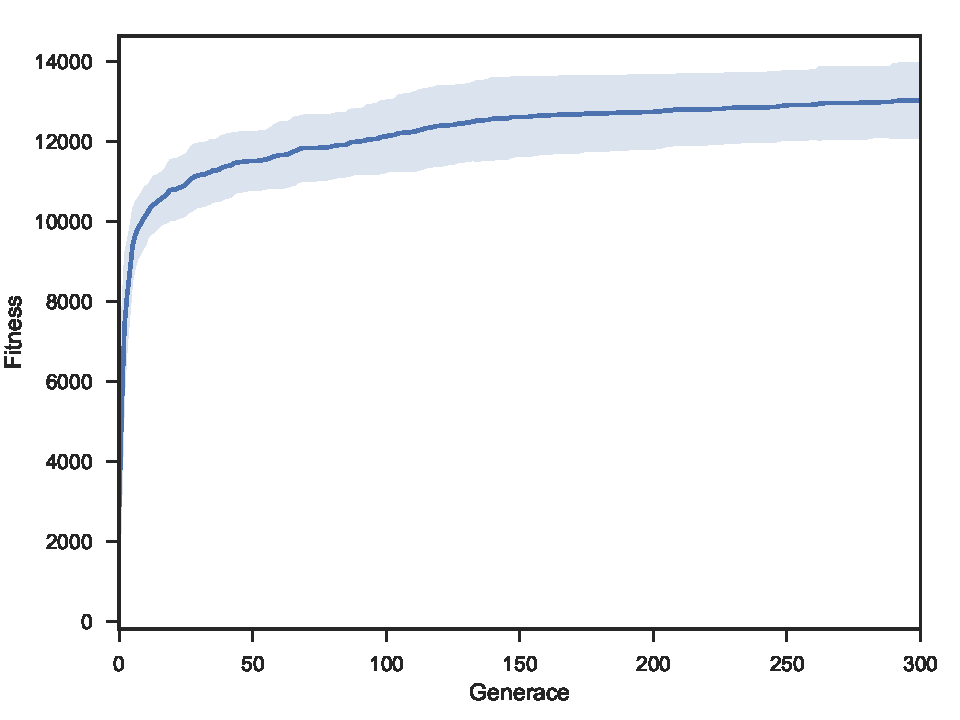
\includegraphics[width=\columnwidth]{../img/MineralMap/MineralWorkerPickup}
	\caption{Mineral Worker sbírání - průběh fitness}
	\label{obr04:MineralWorkerPickUp}
\end{figure}
\clearpage

\subsubsection{Worker skládání - nastavení experimentu}
V dalším metaúkolu jsem se soustředil výhradně na skládání minerálů do středu na místo označeném kódem 2. Konkrétní nastavení experimentu popisuje jako tabulka \ref{tab04:MineralWorkerStore}. Oproti předchozímu scénáři optimalizuji Workery v plném počtu, aby se optimalizovala komunikace a rozptylování Worker robotů. 
\par  
\begin{table}[h]\centering   
	\begin{tabular}{l@{\hspace{1.5cm}}D{.}{,}{3.2}D{.}{,}{1.2}D{.}{,}{2.3}}
		\toprule
		\textbf{Nastavení mapy a EA}\\
		\midrule
		Roboti: & Worker-4\\
		Počet generací: & 6000\\
		Počet iterací map & 1000\\
		Velikost generace(DE) & 100\\
		\bottomrule
		\multicolumn{2}{l}{}
	\end{tabular}
	\par 
	\begin{tabular}{l@{\hspace{1.5cm}}D{.}{,}{3.2}D{.}{,}{1.2}D{.}{,}{2.3}}
		\toprule
		\textbf{Fitness funkce}\\
		\midrule
		Pomocný rádiový signál: & Ano\\
		Hodnota nalezeného minerálu &  1\\
		Hodnota minerálu v pomoc. signálu & 1000\\ 
		Hodnota uložených minerálů & 10\\
		Ostatní hodnoty: & 0\\
		Počet minerálů: & 400\\
		Počet překážek & 100\\
		Počet paliva & 100\\
		\bottomrule
		\multicolumn{2}{l}{}
	\end{tabular}
	\caption{Mineral Worker skládání - nastavení experimentu}
	\label{tab04:MineralWorkerStore}
\end{table}
Výsledek tohoto podúkolu odpovídá Wood Scene - sbírání, roboti dokázali do středu převést přibližně 10 minerálů, opět měli obtíže s uspořádáním. Vizuální výsledek potvrzuje graf \ref{obr04:MineralWorkerStore}.
\clearpage
\begin{figure}[t]\centering
	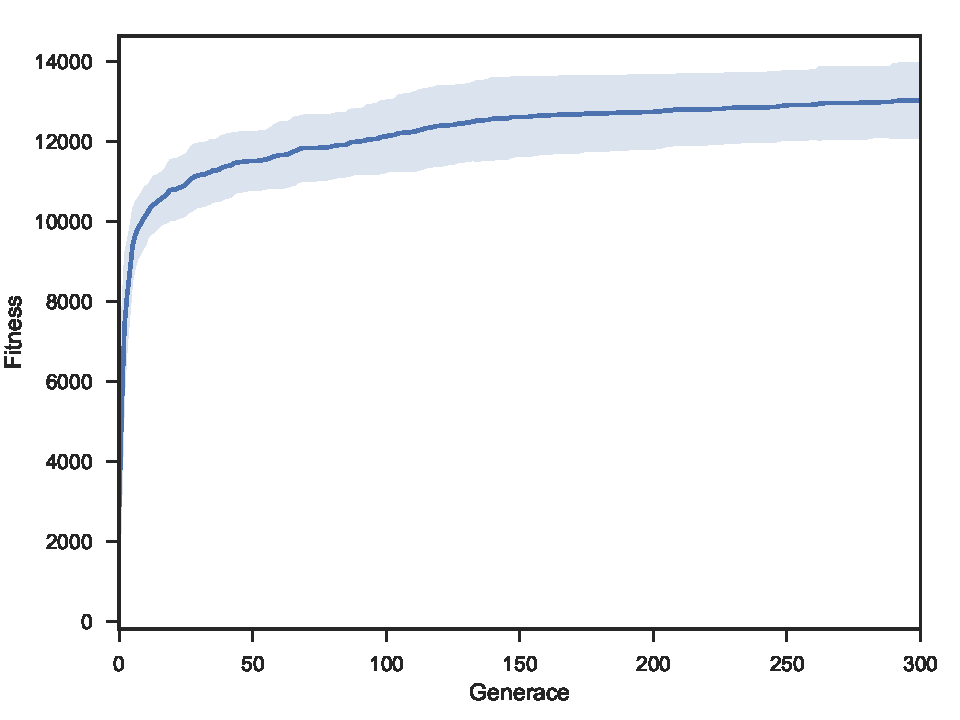
\includegraphics[width=\columnwidth]{../img/MineralMap/MineralWorkerPickup}
	\caption{Mineral Worker skládání -  průběh fitness DE}
	\label{obr04:MineralWorkerStore}
\end{figure}
\clearpage

\subsubsection{Refaktor chůze - nastavení experimentu}
Poslední metaúkol zabývající chůzí byl pro Refaktor robota i v jeho případě byl hodnocen podle počtu nalezených minerálů jako u ostatních robotů. Tabulka \ref{obr04:MineralRefaktorWalk} ukazuje přesné nastavení metaúkolu.
\par
\begin{table}[h]\centering   
	\begin{tabular}{l@{\hspace{1.5cm}}D{.}{,}{3.2}D{.}{,}{1.2}D{.}{,}{2.3}}
		\toprule
		\textbf{Nastavení mapy a EA}\\
		\midrule
		Roboti: & Refaktor-3\\
		Počet generací: & 1000\\
		Počet iterací map & 1500\\
		Velikost generace(DE) & 100\\
		\bottomrule
		\multicolumn{2}{l}{}
	\end{tabular}
	\par 
	\begin{tabular}{l@{\hspace{1.5cm}}D{.}{,}{3.2}D{.}{,}{1.2}D{.}{,}{2.3}}
		\toprule
		\textbf{Fitness funkce}\\
		\midrule
		Hodnota nalezeného minerálu &  1\\
		Ostatní hodnoty: & 0\\
		Počet minerálů: & 500\\
		Počet překážek & 100\\
		Počet paliva & 100\\
		\bottomrule
		\multicolumn{2}{l}{}
	\end{tabular}
	\caption{Mineral Refaktor chůze - nastavení experimentu}
	\label{tab04:MineralRefaktorWalk}
\end{table}
Už v 200 generaci dokážou Refaktor robot odhalí jednu pětinu minerálů, jak je vidět v průběhu grafu na \ref{obr04:MineralRefaktorWalk}. Ač podle fitness se zdá, že roboti prohledávají mapu a vyhýbají se překážkám. Po krátkém zkoumání jejich chování jsem zjistil, že používají nakladače a přehazují překážky za sebe.

\begin{figure}[h]\centering
	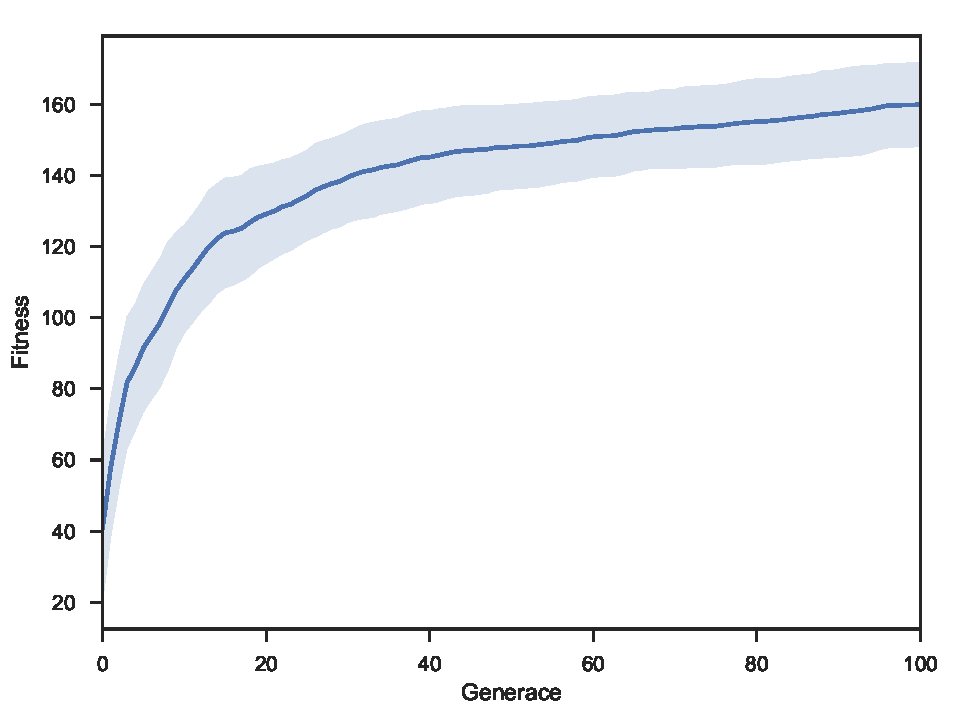
\includegraphics[width=\columnwidth]{../img/MineralMap/MineralRefaktorWalk}
	\caption{Mineral Refaktor chůze - průběh fitness u DE}
	\label{obr04:MineralRefaktorWalk}
\end{figure}
\clearpage

\subsubsection{Refaktor Worker kooperace - nastavení experimentu}
Jako první kooperativní metaúkol jsem zvolil spolupráci Refaktor robota s Workera robota. Zamýšlel 
\begin{table}[h]\centering   
	\begin{tabular}{l@{\hspace{1.5cm}}D{.}{,}{3.2}D{.}{,}{1.2}D{.}{,}{2.3}}
		\toprule
		\textbf{Nastavení mapy a EA}\\
		\midrule
		Roboti: & Refaktor-1, Worker-2\\
		Počet generací: & 2000\\
		Počet iterací map & 1500\\
		Velikost generace(DE) & 100\\
		Počet jedinců(ES) & 10\\
		Počet mutovaný potomků(ES)&10\\
		\bottomrule
		\multicolumn{2}{l}{}
	\end{tabular}
	\par 
	\begin{tabular}{l@{\hspace{1.5cm}}D{.}{,}{3.2}D{.}{,}{1.2}D{.}{,}{2.3}}
		\toprule
		\textbf{Fitness funkce}\\
		\midrule
		Hodnota uložených minerálů & 1\\
		Hodnota přeměného paliva & 1000\\ 
		Hodnota paliva v nádržích & 1000\\
		Ostatní hodnoty: & 0\\
		Počet minerálů: & 400\\
		Počet překážek & 100\\
		Počet paliva & 0\\
		\bottomrule
		\multicolumn{2}{l}{}
	\end{tabular}
	\caption{Mineral Refaktor Worker kooperace - nastavení experimentu}
	\label{tab04:MineralRefactorWorkerCoop}
\end{table}
\redo{Přidat porovnání a výsledky ES}
\clearpage
\begin{figure}[t]\centering
	
\includegraphics[width=\columnwidth]{../img/todo}
	\caption{Mineral Refaktor Worker kooperace - porovnání průběhu fitness ES a DE}
	\label{obr04:MineralRefactorWorkerCoop}
\end{figure}
\redo{Přidat další}
\clearpage

\subsection{Výsledky Experimentu}
\redo{TODO}
\begin{table}[h]\centering   
	\begin{tabular}{l@{\hspace{1.5cm}}D{.}{,}{3.2}D{.}{,}{1.2}D{.}{,}{2.3}}
		\toprule
		& \mc{} & \mc{}\\
		\textbf{Inicializační nastavení:}  \\
		\midrule
		Výška & 800\\ 
		Šířka & 1200\\
		Počet iterací & 10000\\
		Počet stromů & 400\\
		Počet Scout robotů & 5\\
		Počet Worker robotů & 4\\
		\bottomrule
		\multicolumn{2}{l}{}
	\end{tabular}
	\caption{WoodScene - nastavení mapy pro testovací experiment}
\end{table}
\begin{table}[h]\centering   
	\begin{tabular}{l@{\hspace{1.5cm}}D{.}{,}{3.2}D{.}{,}{1.2}D{.}{,}{2.3}}
		\toprule
		& \mc{} & \mc{}\\
		\textbf{Výsledky} \\
		\bottomrule
		Zpracované dřevo zanechané v mapě & 225.22\\
		Stromy v mapě & 156.22\\
		Z toho nalezené & 52.84\\
		Dřevo v kontejnerech & 18.48\\
		Uskladněné dřevo & 17.56\\
		\multicolumn{2}{l}{}
	\end{tabular}
	\caption{WoodScene - výsledky simulace nejlepšího jedince, průměr ze 100 simulací testovacího experimentu}
	\label{tab04:MineralStat}
\end{table}
\newpage 
\begin{figure}[p]\centering
	
\includegraphics[width=\columnwidth]{../img/todo}
	\caption{Nejlepší jedinec - 10000 iterací simulace}
	\label{obr04:MineralBestEnd}
\end{figure}
\begin{figure}[p]\centering
	
\includegraphics[width=\columnwidth]{../img/todo}
	\caption{Náhodný jedinec - 10000 iterací simulace}
	\label{obr04:MineralRandom end}
\end{figure}
\clearpage
\clearpage
\section{Competitive Scene}
Poslední ze scénářů se týká soutěže dvou týmů(hejn) ve kterých figurují jeden malý průzkumný robot(Competitive Scout) a jeden vetší bojový robot(Competitive Fighter). Úspěšnost týmu je dána zachovanými jednotkami zdraví robotů a uděleným poškozením do nepřátelské skupiny robotů. Competitive Scout se pohybuje značně rychleji než Competitive Fighter, ale uděluje menší poškození. Což lze opět vztáhnout na chování rozdílných skupin nepřátel např. ve strategických hrách, kde se jejich chování adaptuje, co nejlépe na dané prostředí. 

\redo{Upravit dle dosáhnuté formy}
\clearpage

\begin{figure}[p]\centering
	
\includegraphics[width=\columnwidth]{../img/todo}
	\caption{Příklad Competitive Scene mapy: start náhodného chování}
	\label{obr04:CompetitiveSceneRandomStart}
\end{figure}
\clearpage 

\subsection{Roboti}

\redo{Obecný popis robotů}
\subsubsection{Fighter Scout robot}
\par  
\begin{table}[h]\centering
	\begin{tabular}{l@{\hspace{1.0cm}}D{.}{,}{2.2}D{.}{,}{2.2}D{.}{,}{2.3}}
		\toprule
		\textbf{Fighter Scout Robot} \\
		\midrule
		Tvar: & Kruh\\
		Poloměr: & 2,5\\
		Namespace: & CompetitiveRobots\\
		Název: & FighterScoutRobotMem \\
		Velikost kontejneru: & 0\\
		\midrule
		\textbf{Efektory} \\
		\midrule
		Motor: & Dvou kolečkový \\
		Maximální rychlost: & 3 \\
		Kód rádiového signálu: & 0,1,2\\
		Poloměr signálu: & 200\\
		Počet paměťových slotů: &10 \\
		Obsah slotu: & float\\
		Počet zbraní: & 3\\
		Dosah zbraní: & 10\\
		Orientace zbraní: &  0^\circ, 45^\circ, -45^\circ\\
		Útok zbraní: & 100\\
		\midrule
		\textbf{Senzory} \\
		\midrule
		Počet line senzorů: &  3\\
		Délka line senzorů: & 70\\
		Orientace l. senzorů: & 0^\circ, 45^\circ, -45^\circ\\
		Poloměr rádiového přijímače: & 100 \\
		Poloměr type senzoru: & 50\\
		Počet touch senzorů: & 3 \\  
		Lokátorový senzor\\ 
		\bottomrule
		\multicolumn{2}{l}{}
	\end{tabular}
	\caption{Competitive Scene - Fighter Scout robot popis }
	\label{tab04:CompetiveScout}
\end{table}
\clearpage
\subsubsection{Fighter robot}
\par  
\begin{table}[h]\centering
	\begin{tabular}{l@{\hspace{1.0cm}}D{.}{,}{2.2}D{.}{,}{2.2}D{.}{,}{2.3}}
		\toprule
		\textbf{Fighter Scout Robot} \\
		\midrule
		Tvar: & Kruh\\
		Poloměr: & 5\\
		Namespace: & CompetitiveRobots\\
		Název: & FighterRobotMem \\
		Velikost kontejneru: & 0\\
		\midrule
		\textbf{Efektory} \\
		\midrule
		Motor: & Dvou kolečkový \\
		Maximální rychlost: & 1,5 \\
		Kód rádiového signálu: & 0,1,2\\
		Poloměr signálu: & 200\\
		Počet paměťových slotů: &10 \\
		Obsah slotu: & float\\
		Počet zbraní: & 4\\
		Orientace zbraní: &  0^\circ, 45^\circ, -45^\circ, 180^\circ\\
		Útok zbraní: & 500\\
		\midrule
		\textbf{Senzory} \\
		\midrule
		Počet line senzorů: &  3\\
		Délka line senzorů: & 70\\
		Orientace l. senzorů: & 0^\circ, 45^\circ, -45^\circ\\
		Poloměr rádiového přijímače: & 100 \\
		Poloměr type senzoru: & 50\\
		Počet touch senzorů: & 3 \\  
		Lokátorový senzor\\ 
		\bottomrule
		\multicolumn{2}{l}{}
	\end{tabular}
	\caption{Competitive Scene - Fighter robot popis }
	\label{tab04:CompetitiveScene}
\end{table}
\clearpage
\subsection{Vyhodnocování Fitness}
\begin{enumerate}
	\item \textit{nalezené stromy} - stromy o které zavadil line senzor 
	\item \textit{pokácené stromy} - stromy, které refaktor změnil 
	\item \textit{sebrané dřevo} - zpracované dřevo, které mají roboti uvnitř kontejnerů 
	\item \textit{uskladněné dřevo} - dřevo, které dovezli na vyznačené místo 
\end{enumerate}
Trestáni za:
\begin{enumerate}
	\item \textit{kolize} - počet pokusů o pohyb při kterém by došlo ke kolizi 
	\item \textit{sebrané entity mimo dřevo} - počet entit v kontejnerech, které nejsou zpracované dřevo 
\end{enumerate}

\subsection{Podúkoly} 
\clearpage

\subsubsection{Scout chůze - nastavení experimentu}

\begin{table}[h]\centering   
	\begin{tabular}{l@{\hspace{1.5cm}}D{.}{,}{3.2}D{.}{,}{1.2}D{.}{,}{2.3}}
		\toprule
		\textbf{Nastavení mapy a EA}\\
		\midrule
		Roboti: & Scout-5 \\
		Počet generací: & 1000\\
		Počet iterací map & 1000\\
		Velikost generace(DE) & 100\\
		Počet jedinců(ES) & 10\\
		Počet mutovaný potomků(ES)&10\\
		\bottomrule
		\multicolumn{2}{l}{}
	\end{tabular}
	\par 
	\begin{tabular}{l@{\hspace{1.5cm}}D{.}{,}{3.2}D{.}{,}{1.2}D{.}{,}{2.3}}
		\toprule
		\textbf{Fitness funkce}\\
		\midrule
		Hodnota nalezeného minerálu &  100 \\
		Ostatní hodnoty: & 0\\
		Počet minerálů: & 400\\
		Počet překážek & 100\\
		Počet paliva & 100\\
		\bottomrule
		\multicolumn{2}{l}{}
	\end{tabular}
	\caption{Scout chůze - nastavení experimentu}
	\label{tab04:CompetitiveWalk}
\end{table}
\redo{TODO}
\clearpage
\subsection{Výsledky Experimentu}
\redo{TODO}
\begin{table}[h]\centering   
	\begin{tabular}{l@{\hspace{1.5cm}}D{.}{,}{3.2}D{.}{,}{1.2}D{.}{,}{2.3}}
		\toprule
		& \mc{} & \mc{}\\
		\textbf{Inicializační nastavení:}  \\
		\midrule
		Výška & 800\\ 
		Šířka & 1200\\
		Počet iterací & 10000\\
		Počet stromů & 400\\
		Počet Scout robotů & 5\\
		Počet Worker robotů & 4\\
		\bottomrule
		\multicolumn{2}{l}{}
	\end{tabular}
	\caption{WoodScene - nastavení mapy pro testovací experiment}
\end{table}
\begin{table}[h]\centering   
	\begin{tabular}{l@{\hspace{1.5cm}}D{.}{,}{3.2}D{.}{,}{1.2}D{.}{,}{2.3}}
		\toprule
		& \mc{} & \mc{}\\
		\textbf{Výsledky} \\
		\bottomrule
		Zpracované dřevo zanechané v mapě & 225.22\\
		Stromy v mapě & 156.22\\
		Z toho nalezené & 52.84\\
		Dřevo v kontejnerech & 18.48\\
		Uskladněné dřevo & 17.56\\
		\multicolumn{2}{l}{}
	\end{tabular}
	\caption{WoodScene - výsledky simulace nejlepšího jedince, průměr ze 100 simulací testovacího experimentu}
	\label{tab04:CompetitiveStat}
\end{table}
\newpage
\begin{figure}[p]\centering
	
\includegraphics[width=\columnwidth]{../img/todo}
	\caption{Nejlepší jedinec - 10000 iterací simulace}
	\label{obr04:CompetitiveBestEnd}
\end{figure}
\begin{figure}[p]\centering
	
\includegraphics[width=\columnwidth]{../img/todo}
	\caption{Náhodný jedinec - 10000 iterací simulace}
	\label{obr04:CompetitiveRandom end}
\end{figure}
\clearpage
\section{Shrnutí}